\documentclass[oneside]{article}
\usepackage[backend=biber,natbib=true,style=authoryear]{biblatex}
\addbibresource{~/1_PROJECTS/GitHub/math-lecture-notes/NQBH_Bibliographies.bib}
\usepackage[utf8]{inputenc}
\usepackage{graphicx}
\usepackage[colorlinks=true,linkcolor=blue,urlcolor=red,citecolor=magenta]{hyperref}
% Math
\usepackage{amsmath,amssymb,amsthm}
\allowdisplaybreaks
\numberwithin{equation}{section}
\numberwithin{figure}{section}

\newtheorem{assumption}{Assumption}[section]
\newtheorem{lemma}{Lemma}[section]
\newtheorem{corollary}{Corollary}[section]
\newtheorem{definition}{Definition}[section]
\newtheorem{proposition}{Proposition}[section]
\newtheorem{theorem}{Theorem}[section]
\newtheorem{notation}{Notation}[section]
\newtheorem{remark}{Remark}[section]
\newtheorem{example}{Example}[section]
\newtheorem{ques}{Question}[section]
\newtheorem{problem}{Problem}[section]
\newtheorem{conjecture}{Conjecture}[section]
% Layout
\usepackage[left=0.5in,right=0.5in,top=1.5cm,bottom=1.5cm]{geometry}
\usepackage{lscape} % landscape format

\newcommand{\TT }{ \mathcal{T}}
%
\newcommand{\e }{ \varepsilon}
\newcommand{\om }{ \omega}
\newcommand{\Om }{ \Omega}
\newcommand{\de }{ \delta}
\newcommand{\dn }{ \partial_n}
\newcommand{\dna }{ \partial_{n_1}}
\newcommand{\dnb }{ \partial_{n_2}}
\newcommand{\dnx }{ \partial_{n_x}}
\newcommand{\dnxi }{ \partial_{n_\xi}}
\newcommand{\curl }{ \nabla \times}
\newcommand{\ue }{u_{\e,\gamma}}
\newcommand{\pe }{p_{\e,\gamma}}
\newcommand{\s}{\sum_{j=1}^2}
\newcommand{\Dj }{ \partial_j}
\newcommand{\gj}{\mathcal{G}_j}
\newcommand{\bg}{\bar{g}}
\newcommand{\hL}{\hat{L}}
\newcommand{\hQ}{\hat{Q}}
\newcommand{\hM}{\hat{M}}
\newcommand{\hu}{\hat{u}}
\newcommand{\hx}{\hat{x}}
\newcommand{\hq}{\hat{q}}
\newcommand{\tu}{\tilde{u}}
\newcommand{\tq}{\tilde{q}}
\newcommand{\tphi}{\tilde{\phi}}
\newcommand{\bu}{\bar{u}}
\newcommand{\ou}{\overline{u}}
\newcommand{\uu}{\underline{u}}
\newcommand{\tw}{\tilde{w}}
\newcommand{\hw}{\hat{w}}
\newcommand{\hS}{\hat{S}}
\newcommand{\hbF}{\hat{\boldsymbol{F}}}
\newcommand{\tG}{\tilde{G}_\delta}
\newcommand{\ti}{\tilde{I}_\delta}
\newcommand{\tyd}{\tilde{y}_\delta}
\newcommand{\A }{ \mathcal{A}}
\newcommand{\HH }{ \mathcal{H}}
\newcommand{\B }{ \mathcal{B}}
\newcommand{\C }{ \mathcal{C}}
\newcommand{\I }{ \mathcal{I}}
\newcommand{\Ie }{ \mathcal{I}_{\e,\gamma}}
\newcommand{\Ae }{ \mathcal{A}_{\e,\gamma}}
\newcommand{\Be }{ \mathcal{B}_{\e,\gamma}}
\newcommand{\T }{ \mathcal{T}}
\newcommand{\OO }{ \mathcal{O}}
\newcommand{\KK }{ \mathcal{K}}
\newcommand{\N }{ \mathcal{N}}
\newcommand{\R }{ \mathcal{R}}
\newcommand{\RR }{ \mathbb{R}}
\newcommand{\Sh }{ \mathcal{S}}
\newcommand{\xx}{\emph{\textbf{x}}}
\newcommand{\xxx}{\textbf{x}}
\newcommand{\nn}{\textbf{n}}
\newcommand{\buu}{\boldsymbol{u}}
\newcommand{\bFF}{\boldsymbol{F}}
\newcommand{\bQQ}{\boldsymbol{Q}}
\newcommand{\baa}{\boldsymbol{a}}
\newcommand{\bxx}{\boldsymbol{x}}
\newcommand{\brr}{\boldsymbol{r}}
\newcommand{\byy}{\boldsymbol{y}}
\newcommand{\bbb}{\boldsymbol{b}}
\newcommand{\bww}{\boldsymbol{w}}
\newcommand{\bgg}{\boldsymbol{g}}
\newcommand{\bbuu}{\bar{\boldsymbol{u}}}
\newcommand{\bnn}{\boldsymbol{n}}
\newcommand{\bcc}{\boldsymbol{n}}
\newcommand{\bdd}{\boldsymbol{d}}
\newcommand{\bzz}{\boldsymbol{0}}
\newcommand{\oa}{\Om_1^\e}
\newcommand{\ob}{\Om_2^\e}
\newcommand{\ua}{u_1^\e}
\newcommand{\ub}{u_2^\e}
\newcommand{\ra}{\mathcal{R}_{2,\e}^1}
\newcommand{\raa}{\mathcal{R}_{1,\e}^1}
\newcommand{\sa}{\mathcal{S}_{2,\e}^1}
\newcommand{\saa}{\mathcal{S}_{1,\e}^1}
\newcommand{\rb}{\mathcal{R}_{2,\e}^2}
\newcommand{\Sb}{\mathcal{S}_{2,\e}^2}
\newcommand{\LL }{ \mathcal{L}}
\newcommand{\DD }{ \mathcal{D}}
\newcommand{\JJ }{ \mathcal{J}}
\newcommand{\SSg }{ \mathcal{SG}}
\newcommand{\PP }{ \mathcal{P}}
\newcommand{\hJJ }{ \hat{\mathcal{J}}}
\newcommand{\hJ }{ \hat{J}}
%
\newcommand{\uup }{ \buu' }
\newcommand{\ppp }{ \bpp' }
\newcommand{\pp }{ p' }
\newcommand{\phip }{ \phi' }
\newcommand{\zp }{ \bz' }
%
\newcommand{\bvv}{\boldsymbol{v}}
\newcommand{\bUU}{\boldsymbol{U}}
\newcommand{\btau}{\boldsymbol{\tau}}

%
\newcommand{\bpp}{\boldsymbol{p}}
\newcommand{\bz}{\boldsymbol{z}}
\newcommand{\bx}{\boldsymbol{x}}

\newcommand{\bvt}{\tilde{\bvv}}
\newcommand{\but}{\tilde{\buu}}
\newcommand{\bxt}{\tilde{\bxx}}
\newcommand{\bxb}{\bar{\bxx}}
%
\newcommand{\yu}{\byy^{\buu}}

\numberwithin{figure}{section}
\usepackage[table]{xcolor}  
\renewcommand{\qedsymbol}{$\blacksquare$}
\definecolor{light-gray}{gray}{0.7}
\definecolor{dark-gray}{gray}{0.4}
\definecolor{orange}{rgb}{1,0.5,0}
%
\definecolor{dgreen}{rgb}{0.,0.6,0.}
\definecolor{dred}{rgb}{0.6,0.,0.}
\definecolor{dorange}{rgb}{0.9,0.5,0.}
\definecolor{dblue}{rgb}{0.,0.,0.6}
\definecolor{grey}{rgb}{0.5,0.5,0.5}

\title{Handbook for Software\\
Shape- and Topology Optimization}
\date{\today}

\begin{document}
\maketitle
\begin{itemize}
    \item Prof. Dr. M. Hintermüller (Humboldt-Universität zu Berlin)
    \item Dr. K. Knall (Mathtec, Wien)
    \item MMag. M. Kanitsar (Mathtec, Wien/Universität Graz)
\end{itemize}
Software-Version: 1612.
\setcounter{secnumdepth}{6}
\setcounter{tocdepth}{6}
\tableofcontents

\section{Installation}

\subsection{Folder structuring and compilation of the applications}
To use the shape and topology optimizations, the standard installation of OpenFOAM \verb|$FOAM_APP/solvers/incompressible/| must be extended by the following applications:
\begin{itemize}
    \item \texttt{generateFieldsFoam}
    \item \texttt{shapeGradientWall}
    \item \texttt{shapeGradientCCM}
    \item \texttt{setupShapeGradientCCM}
    \item \texttt{shapeGradientAddSTL}
    \item \texttt{shapeGradientCloseAll}
    \item \texttt{topoOpt}
    \item \texttt{topoOptCloseAll}
    \item \texttt{topoExtractSTL}
\end{itemize}
The folder \texttt{InitialSGccm} must be copied into the \verb|$FOAM_RUN/tutorials/| directory. The console commands for installation can be found in the shell-script \texttt{installShapeGradient.sh}.

%------------------------------------------------------------------------------%

\section{Geometry Data}

\subsection{Storage structure of the data in STL format}
The geometry data must be created in the \verb|initial_stl| folder. In addition to the installation space geometry (\texttt{bds.stl}), the surfaces are saved in 4 files in STL format (\texttt{inlet.stl}, \texttt{fixed.stl}, \texttt{wall.stl}, \texttt{outlet.stl}).

The test geometry \textit{M23} with 2 inlets, 3 outlets and an additional fixed geometry (see Table \ref{tab:stlDaten1}) serves as an illustration.

\begin{figure}[htbp]
    \centering
    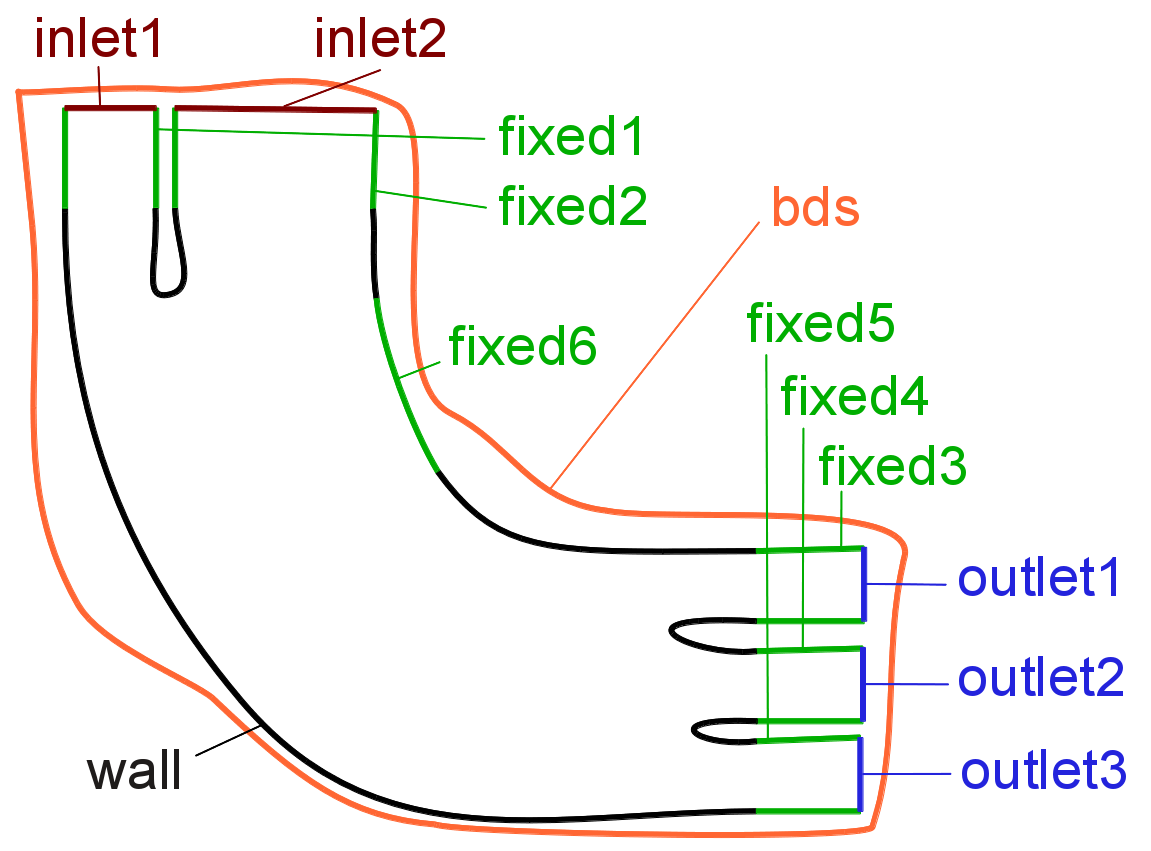
\includegraphics[scale=0.55]{skizze_designSpace4.png}
    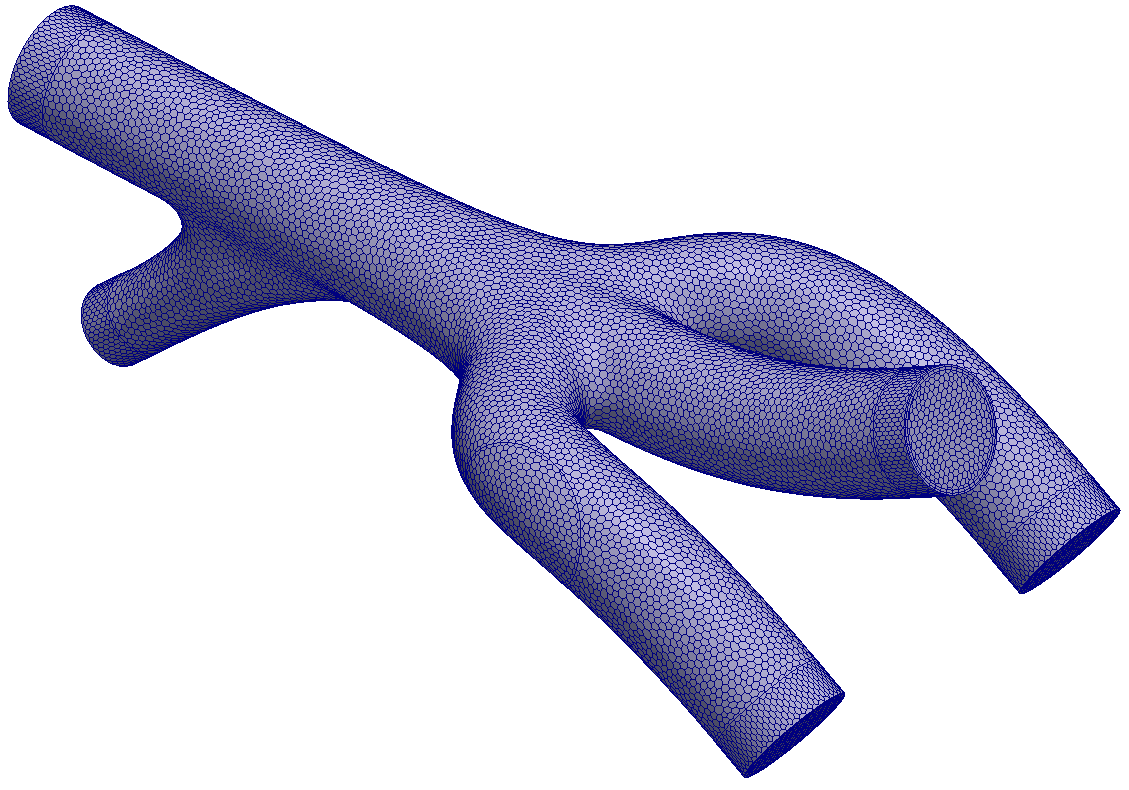
\includegraphics[scale=0.18]{M23all.png}   
    \caption{Left: Sketch geometry data, right: test geometry M23.} 
    \label{fig:sketch building space}
\end{figure}

\begin{table}[h]
    \centering
    \begin{tabular}{|p{0.9cm}|p{4.6cm}|p{3.7cm}|p{1.2cm}|} %lcrp
        \hline
        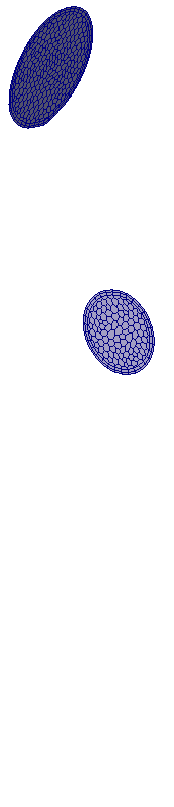
\includegraphics[scale=0.35]{M23in.png}  &  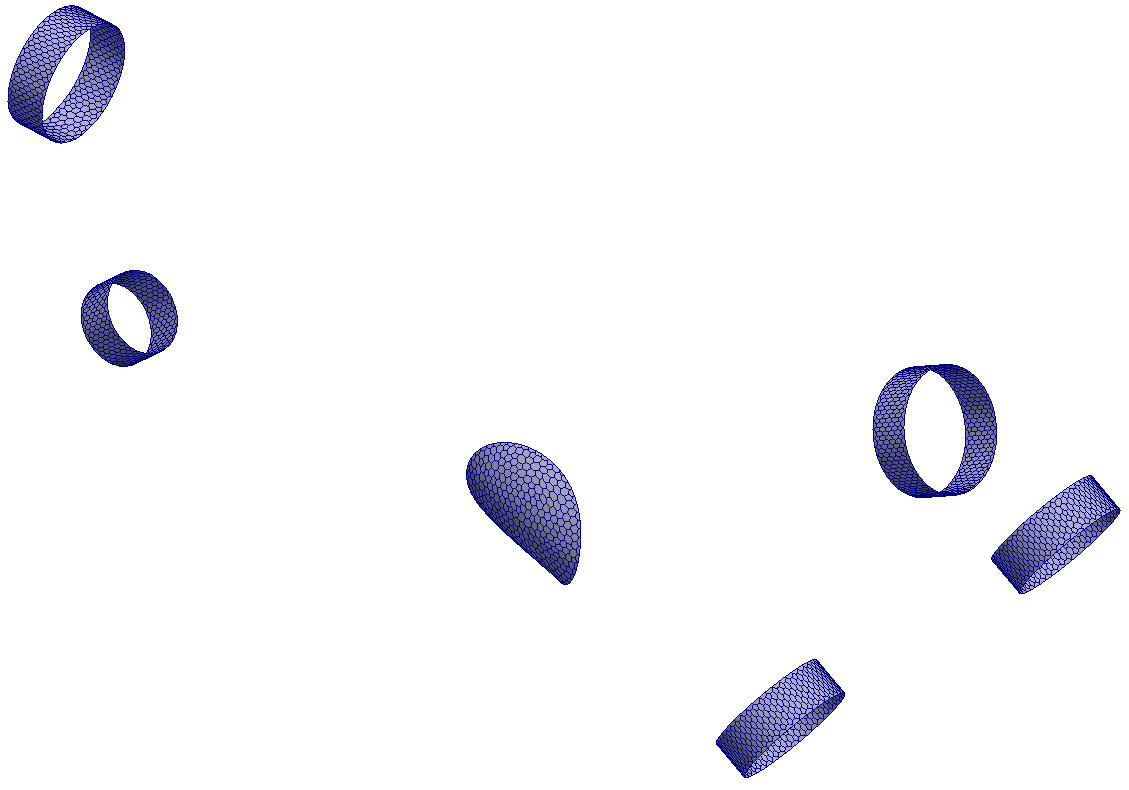
\includegraphics[scale=0.1]{M23fixed.png}   &   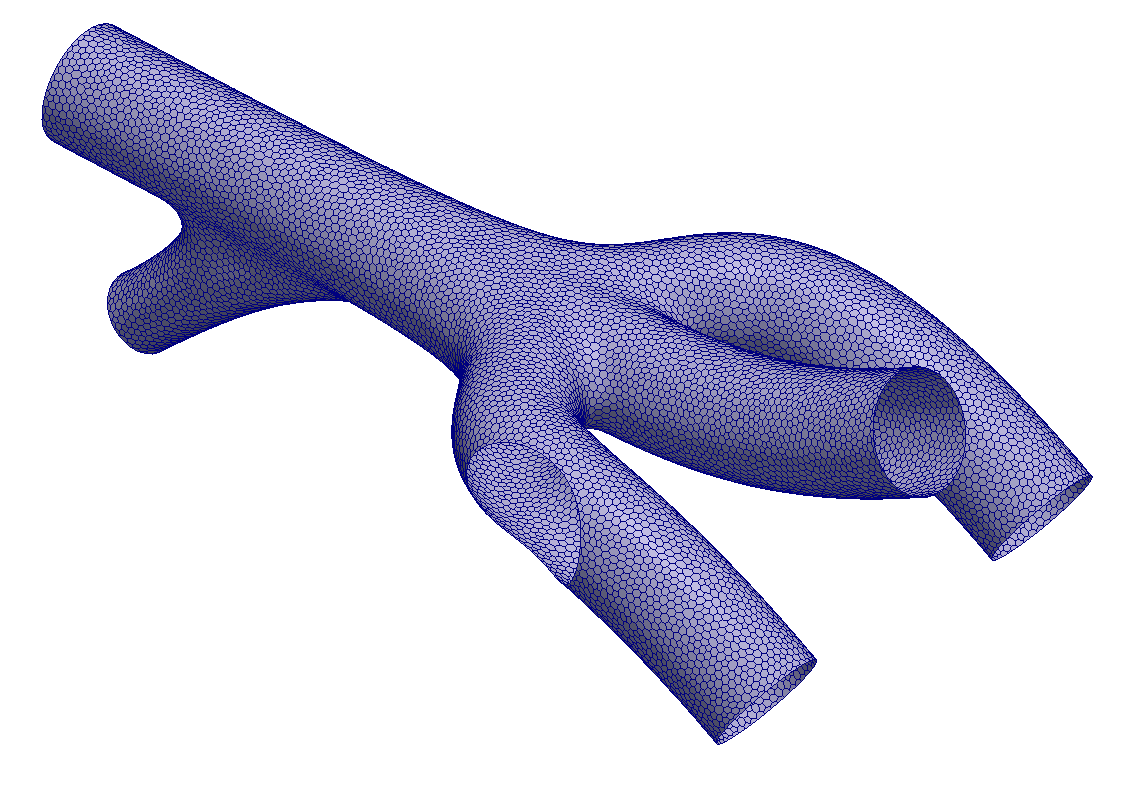
\includegraphics[scale=0.1]{M23wall.png}  &   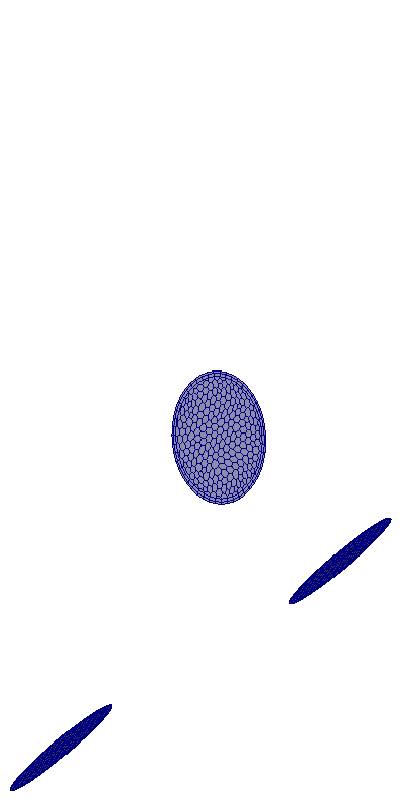
\includegraphics[scale=0.35]{M23out.png}  \\
        \hline
        \textcolor{dred}{inlet.stl}  &  \textcolor{dgreen}{fixed.stl}      &   wall.stl &  \textcolor{dblue}{outlet.stl} \\
        \hline
        \textcolor{dred}{inlet1} \quad \textcolor{dred}{inlet2}  &  
        \textcolor{dgreen}{fixed1} \textcolor{gray}{[inlet1]} ,  \textcolor{dgreen}{fixed2} \textcolor{gray}{[inlet2] \;} 
        \textcolor{dgreen}{fixed3} \textcolor{gray}{[outlet1]} ,  \textcolor{dgreen}{fixed4} \textcolor{gray}{[outlet2]}
        \textcolor{dgreen}{fixed5} \textcolor{gray}{[outlet3]} ,  \textcolor{dgreen}{fixed6}
        &   wall.stl &  \textcolor{dblue}{outlet.stl} \\
        \hline
    \end{tabular}
    \caption{Geometric data in STL format.}\label{tab:stlDaten1}
\end{table}
%
\begin{table}[h]
    \centering
    \begin{tabular}{|p{1.3cm}|p{5.1cm}|p{4cm}|} %lcrp
        \hline
        \cellcolor{light-gray} File name & \cellcolor{light-gray} Designation & \cellcolor{light-gray} Description\\
        \hline
        inlet.stl  &  inlet1, inlet2, inlet3          &   Inflow geometries.\\
        \hline
        outlet.stl  &  outlet1, outlet2, outlet3            &   Outflow geometries.\\
        \hline
        fixed.stl  &  fixed1, fixed2, fixed3, fixed4, fixed5, fixed6, fixed7, fixed8, fixed9 & Geometric data of the fixed areas.\\
        \hline
        wall.stl  &  wall        & Geometric data of the area to be optimized.\\
        \hline
        bds.stl &  bds & Geometric data of the installation space.\\
        \hline
    \end{tabular}
    \caption{Geometric data in STL format.}\label{tab:stlDaten2}
\end{table}
Each inlet and outlet area has a fixed geometry that describes the connection to the geometry to be optimized. Additionally, the user can define fixed geometries which are only connected to the geometry to be optimized (e.g.: \texttt{fixed6} in test geometry \textit{M23}).

The fixed geometries are numbered consecutively, starting with the connections to the inlet geometry, continuing with the connections to the outlet geometry and ending with the fixed geometries that are only connected to the geometry to be shape optimized.

When selecting the installation space geometry, care should be taken to ensure that the start geometry is completely within the allowed range and extends beyond the \verb|inti_freegeom_fixed-inlet| and \verb|into_free-geom_fixed-outlet| interfaces (see Fig. 2.1).

\textsf{Table 2. Geometric data in STL format.}

\texttt{File name}: \textbf{Designation}: \textbf{Description}
\begin{itemize}
    \item \texttt{inlet.stl}: inlet1, inlet2, inlet 3: Inflow geometries.
    \item \texttt{outlet.stl}: outlet1, outlet2, outlet3: Outlet geometries.
    \item \texttt{fixed.stl}: fixed1, fixed2, fixed3, fixed4, fixed5, fixed6, fixed7, fixed8, fixed9: Geometric data of the fixed areas.
    \item \texttt{wall.stl}: wall: Geometric data of the area to be optimized.
    \item \texttt{bds.stl}: bds: Geometric data of the installation space.
\end{itemize}

\subsection{Modeling of the inflow/outflow areas}
The following preparation serves to represent the modeling of an application with regard to the surface geometries of the inflow areas and the outflow areas.

\subsubsection{Inflow areas}
Any number of inlet flow ranges can be defined. An inflow area can also consist of several unconnected geometries. The characteristic of an inlet flow area is not the shape/topology but the physical properties, e.g: face velocity.
\begin{itemize}
    \item Therefore an application with the same inflow velocity can also be modeled with an inflow area (left graph in Fig. 2.2).
    \item If there are different inflow velocities in the application, different inflow ranges must be defined (right graph in Fig. 2.2).
\end{itemize}
\begin{figure}[htbp]
    \centering
    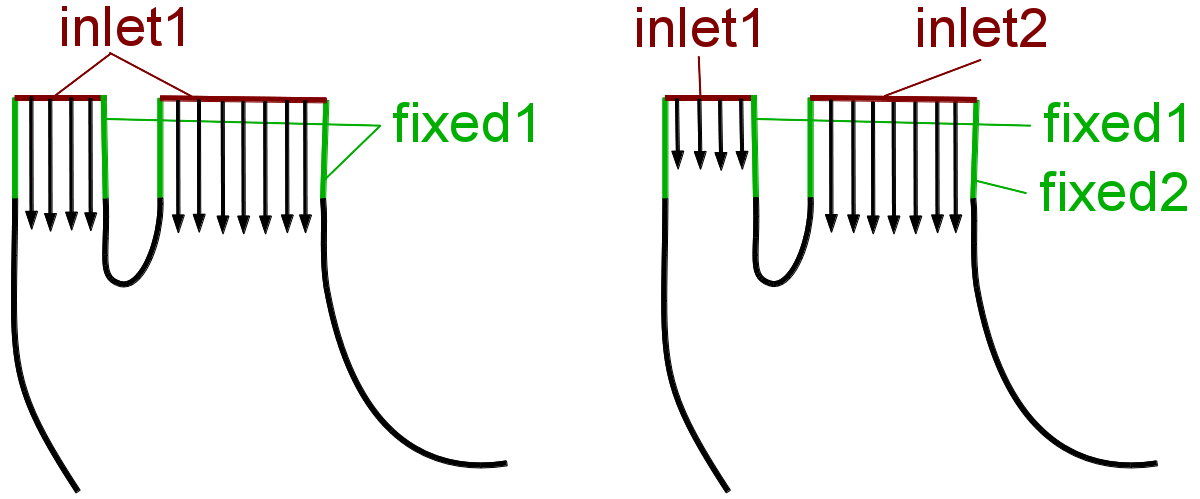
\includegraphics[scale=0.53]{inletMULT.png}   
    \caption{Figure 2.2: Inflow areas.}
    \label{fig:multInlet}
\end{figure}

\subsubsection{Outflow areas}
Any number of discharge ranges can be defined. Analogous to the definition of the inlet flow ranges, the definition of the outlet flow ranges must be made on the basis of the physical properties. In the previous applications, however, the 'do nothing' boundary condition was always used uniformly. The division into different discharge ranges is also relevant if different discharge profiles are desired. Figure 2.3 illustrates the two optimization variants for a uniform flow ($\mathcal{J}_1$).
\begin{figure}[htbp]
    \centering
    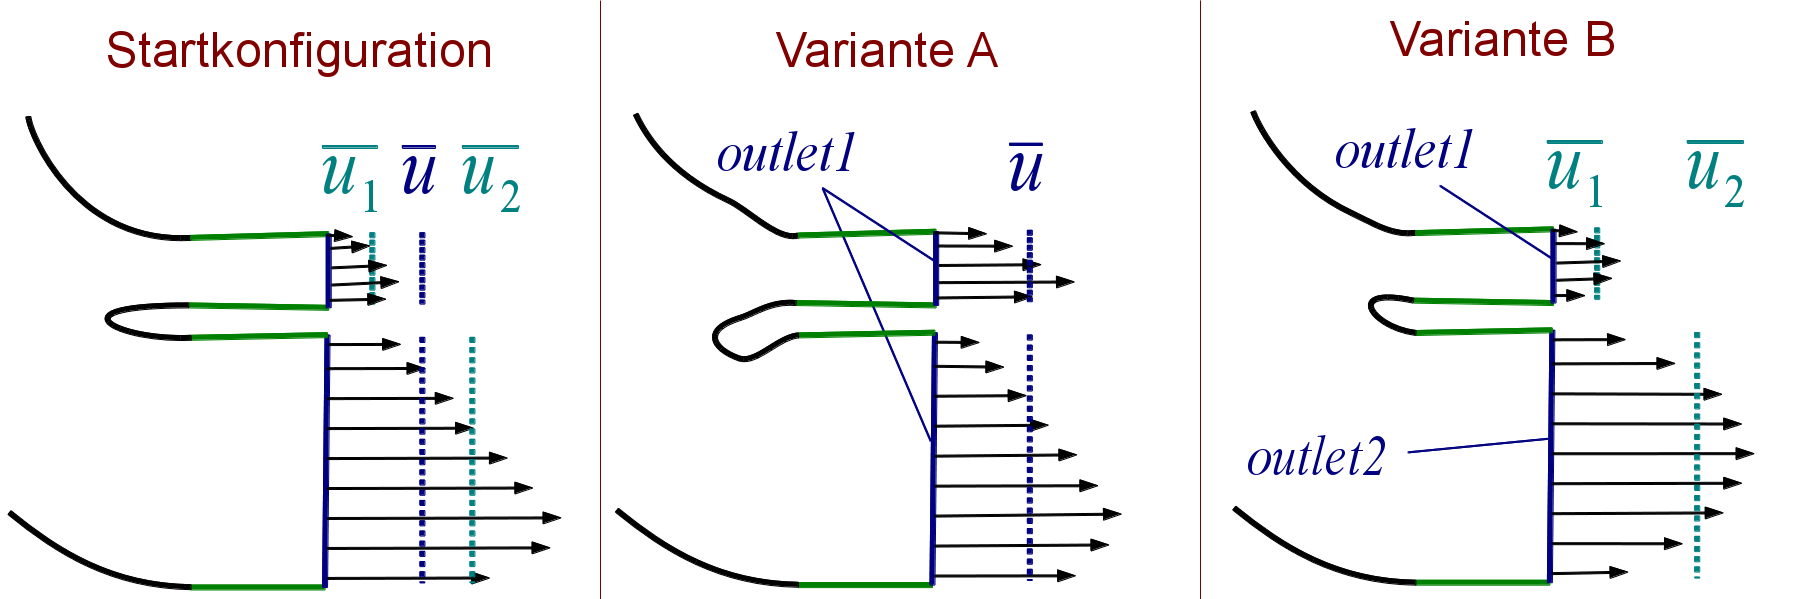
\includegraphics[scale=0.53]{outletMULT.png}   
    \caption{Fig. 2.3: Left: Start. Middle: Optimization $\mathcal{J}_1|_{\Gamma_{\rm out}^1\cap\Gamma_{\rm out}^2}$. Right: Optimization $\gamma_1\mathcal{J}_1|_{\Gamma_{\rm out}^1} + \gamma_2\mathcal{J}_1|_{\Gamma_{\rm out}^2}$.}
    \label{fig:multOutlet}
\end{figure}

\subsection{User defined inflow profile}
If an inflow profile is to be specified, the corresponding entry in the parameter \verb|velocity_ massflow| must be set to 0 and a file \verb|velocity_inletI.csv| with $I = \{0,1,2,\ldots\}$ must be specified in the order of the test calculation. If, in the example M23, a profile is to be specified at the 2nd inflow area, \verb|velocity_massflow| = $2(36.5,0)$ must be set and a file \verb|velocity_inlet2.csv| must be created.

\subsection{Initial geometry Topology optimization}
For topology optimization, the largest possible initial geometry should be specified. Figure 2.4 shows an initial geometry for the application example clean air tube (RLR).
\begin{figure}[htbp]
    \centering
    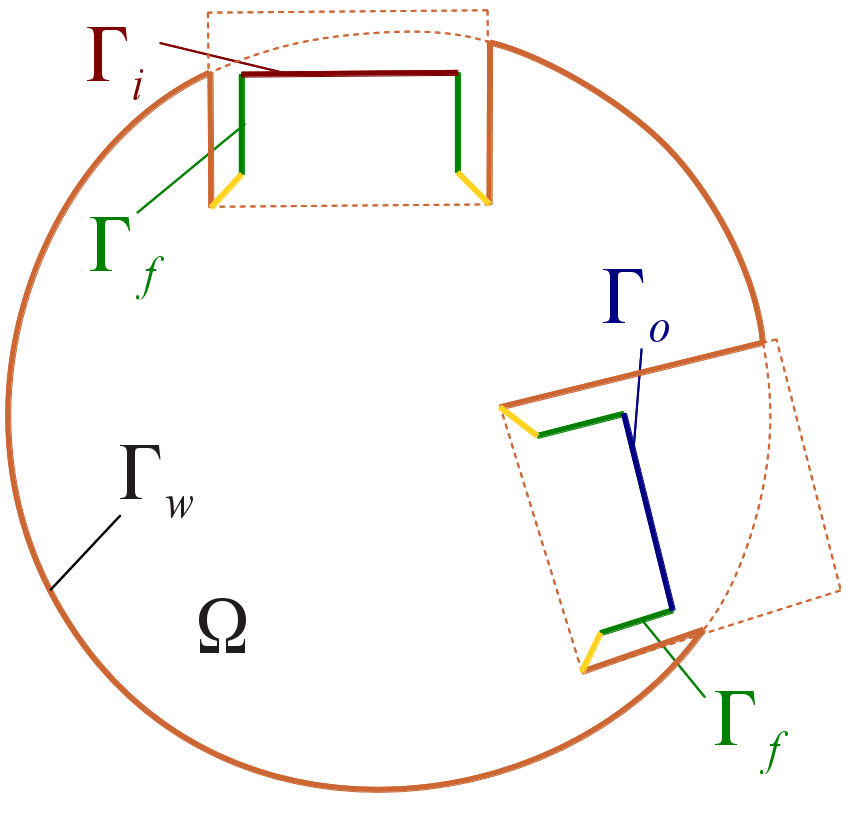
\includegraphics[scale=0.42]{TopoStartgeometrieSkizze.png}
    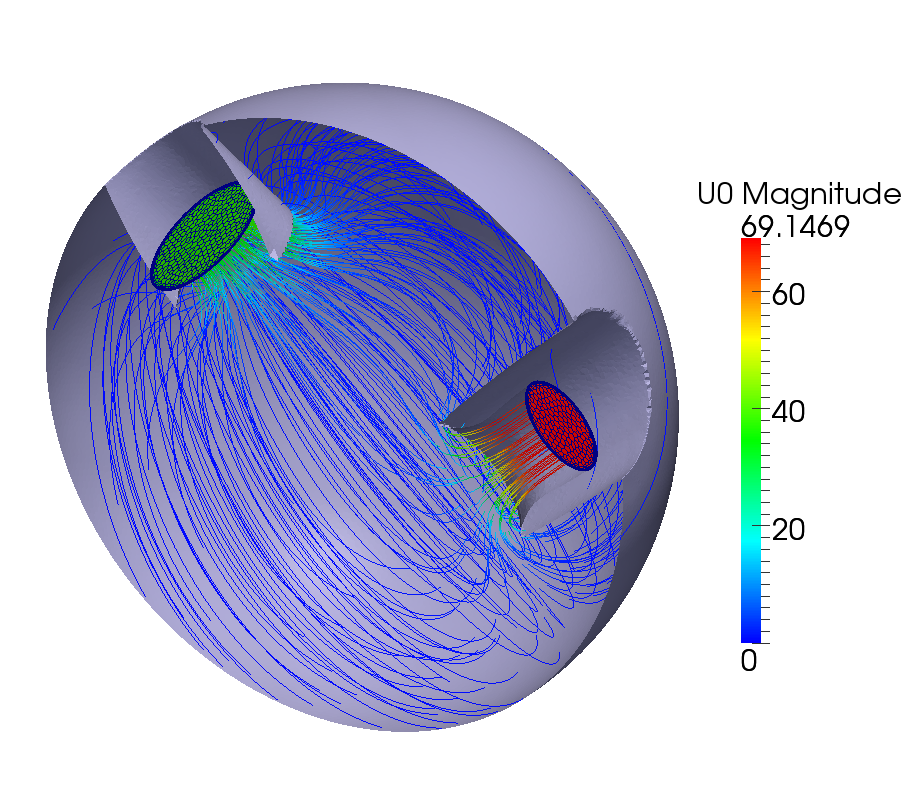
\includegraphics[scale=0.15]{TopoStartgeometrie.png}
    \caption{Figure 2.4: Initial geometry Topology Optimization RLR.}
    \label{AnfangTopo}
\end{figure}

\section{Parameters and their meaning}
In addition to the geometry data, the parameter file \verb|parameter_sg| must be created. The parameters contained in this file are explained in this chapter. The parameters are inserted in the Java scripts \texttt{mbmw3.java, solvePrimal.java} and \texttt{solveAdjoint.java}. If changes are to be made in the Star-CD CCM+ usage, these 3 files in the \texttt{initialSG} folder must be adapted. The parameters relevant for OpenFOAM are stored in \texttt{system/fvSolution} after calling the setup routine.
\begin{table}[h]
    \centering
    \begin{tabular}{|c|c|c|c|c|p{7cm}|}
        \hline
        \cellcolor{light-gray}\textbf{Parameter name} & \cellcolor{light-gray}\textbf{Default value} & \cellcolor{light-gray}\textbf{Admissibility} & \cellcolor{light-gray}\textbf{RLR} & \cellcolor{light-gray}\textbf{M23} & \cellcolor{light-gray}\textbf{Description} \\
        \hline
        \verb|install_location| &  &  &  &  & Path of the star CD CCM+ bin file to start CCM+. \\
        \hline
        \texttt{prozessNumber} & 2 & [1,100] & 2 & 2 & Number of processors with parallelization in Star-CD CCM+.\\
        \hline
    \end{tabular}
    \caption{Parameter Star-CD CCM+.} \label{tab:parameter1}
\end{table}

\subsection{Grid generation}
In Star-CD CCM+ a polyhedron grid is created. The grid fineness is defined by the Reference value for the cell size \verb|base_size| adjustable. The number of inlets and outlets as well as the number of optional fixed surfaces must be specified (\texttt{numInlet, numOutlet, numFixed}). The mesh quality for mesh generation can be increased through the \verb|mesh_opt_cycles| and \verb|mesh_quality_treshold| parameters. Layer layers are to be used near the wall. The size and number of these layers is defined by the \verb|num_layer_wall|, \verb|thick_layer| and \verb|layer_stretch| parameters. To prevent backflow on the outflow geometry (`do-nothing' boundary condition), usually an additional extrusion geometry is required. The adjustment of length and discretization can be done with the parameters \verb|extrude_|... parameters. The grid is locally refined in CCM+ on the basis of the surface condition. If this refinement is not the parameter \verb|grid_local_refinement| is to be set to 0.
\begin{table}[h]
    \centering
    \begin{tabular}{|p{2.1cm}|p{1cm}|p{1.5cm}|p{0.6cm}|p{0.5cm}|p{0.5cm}|p{5.6cm}|} %lcrp
        \hline
        \cellcolor{light-gray} Parameter-name & \cellcolor{light-gray} Default value 
        & \cellcolor{light-gray} Admissibility & \cellcolor{light-gray} RLR & \cellcolor{light-gray} M23 & \cellcolor{light-gray} B135
        & \cellcolor{light-gray} Description \\
        \hline
        base\_size         & 0.004  & [1e-4,0.1]          & 0.004 & 0.03 &  0.04  & Grid fineness: Cell size.\\
        \hline
        numInlet           & 1      & \{1,2,...1e3\}      & 1     &   2  &   1    & Number of inflow areas.\\
        \hline
        numOutlet          & 1      & \{1,2,...1e3\}      & 1     &   3  &   1    & Number of outlet areas.\\
        \hline
        numFixed           & 0      & \{0,1,...1e3\}     & 0     &   1    &   0    & Number of optional fixed geometries.\\
        \hline
        num\_layer\_wall   &   2    & [0,6]              & 2     &   3    &   6    & Number of layer layers at the edge.\\
        \hline
        thick\_layer       &   60   & [10,100]           & 80    &   60   & 60     & Thickness of the layer layers in percent (relative to neighboring cell size).\\
        \hline 
        layer\_stretch     &   1.5  & [1e-3,1e3]         & 1.5   & 1.5    & 1.4    & Magnification factor of the layer layers.\\ 
        \hline
        extrude\_ \qquad \; outlet\_length & 0.05 &  [1e-8,1e8] & 0.06 & 0.2 & 1.2 & Length of the extrusion geometry at the outlet.\\
        \hline
        extrude\_ \qquad \; outlet\_num    & 32   &  [1,1e5]    & 20 & 10   & 90   & Number of cell layers in the extrusion geometry at the outlet.\\
        \hline
        extrude\_ \qquad \; outlet\_stretch & 1   &   [1e-3,1e3]  & 1 & 1   &  1   & Magnification factor of the layers in the extrusion geometry at the outlet.\\
        \hline
        extrude\_ \qquad \; inlet\_length   & 0.025 &   [1e-8,1e8]    & 0.03 & 0.2  & 0.2 & Length of the extrusion geometry at the inlet.\\
        \hline
        extrude\_ \qquad \; inlet\_num      & 16 &   [1,1e5]     & 10 & 10 & 15 & Number of cell layers in the extrusion geometry at the inlet.\\
        \hline
        extrude\_ \qquad \; inlet\_stretch  & 1 &    [1e-3,1e3]      & 1 & 1 & 1 & Magnification factor of the layer layers in the extrusion geometry at the inlet.\\
        \hline
        mesh\_opt\_ \quad cycles        & 8 &   [1,8]     & 8 & 8 & 8 & Polyhedron mesh: Quality optimization loops.\\
        \hline
        mesh\_quality \quad \_treshold  &1&   [0,1]     & 1 & 1 & 1 & Polyhedron mesh: quality optimization barrier.\\
        \hline
        grid\_local\_ \qquad refinement  & 0 &  \{0,1\}    & 0 & 1 & 1 & Local grid refinement: 0:no, 1:yes.\\
        \hline
        ext\_merge  & 0 &  \{0,1\}    & 0 & 1 & 0 & Combine extrusion geometry with fixed geometries: 0:no, 1:yes\\
        \hline
    \end{tabular}
    \caption{Parameters for grid generation in Star-CD CCM+.}\label{tab:parameter1}
\end{table}

\subsection{Model selection and physical settings}
To specify the flow velocity, either a constant inflow velocity in m/s or the mass flow rate in kg/s can be entered (\verb|velocity_massflow_par| = 0 or 1). The values are defined by the parameter \verb|velocity_massflow| to be specified. The corresponding syntax is shown in table \ref{tab:parameter2a}.

Beside the direct numerical simulation (\verb|turb_model| = 0) currently 4 turbulence models can be selected with the parameter \verb|turb_model|. If other turbulence models prove to be suitable for future software versions, the JavaScript \textit{mbmw3.java} must be adapted accordingly. Furthermore, the following model parameters must be specified in Star-CD CCM+: \verb|inlet_turb_intensity|, \verb|inlet_visc_ratio|, \verb|outlet_turb_intensity|, \verb|outlet_visc_ratio|.

\begin{table}[h]
    \centering
    \begin{tabular}{|p{2.8cm}|p{0.9cm}|p{1.5cm}|p{0.8cm}|p{1.0cm}|p{0.7cm}|p{4.3cm}|} %lcrp
        \hline
        \cellcolor{light-gray} Parametername & \cellcolor{light-gray} Default value & \cellcolor{light-gray} Admissibility & \cellcolor{light-gray} RLR & \cellcolor{light-gray} M23  & \cellcolor{light-gray} B135 & \cellcolor{light-gray} Description\\
        \hline
        turb\_model                     &   2           & [0,100]      & 1      & 0               &  4  & 0: DNS, 1: Realiz. k-$\varepsilon$ all Y+, 2: Std. k-$\varepsilon$ high Y+, 3: RSM all Y+, 4: Realiz. k-$\varepsilon$ low Y+.\\
        \hline
        velocity\_massflow\_ \quad par  &   0           & \{0,1\}      & 0      & 0               &  0  & Inflow: 0:velocity, 1:mass flow.\\
        \hline
        velocity\_massflow              &  1(0.1)       &  [1e-8,1e8]  & 1(36.5)& 2(0.006, 0.006) &  1(4.3)  & Inflow (velocity or mass flow)\\
        \hline
        inlet\_turb\_intensity          &  0.1          &  [1e-8,1e8]  & 0.1    &                 &  0.1  & Turbulent Intensity Inlet.\\
        \hline
        inlet\_turb\_length    &   \textcolor{dred}{10} &  [1e-8,1e8]   & 0.1   &                 &   10 & Turbulent Length Scale Inlet.\\
        \hline
        outlet\_turb\_intensity        &  0.1           &  [1e-8,1e8]   & 0.1   &                 &   0.1 & Turbulent Intensity Outlet.\\
        \hline
        outlet\_turb\_length      & \textcolor{dred}{10} &  [1e-8,1e8]  & 0.1   &                 &   10 & Turbulent Length Scale Outlet.\\
        \hline
    \end{tabular}
    \caption{Parameters for physical models.}\label{tab:parameter2a}
\end{table}

\subsection{Solver settings for the primary and adjoint equation}
The solvers in CCM+ use a pseudo time-stepping method. The step size control is to be specified by the Courant-Friedrichs-Lewy number (\texttt{CFLpri, CFLadj}). The choice of a large number allows a faster achievement of the desired solution, but can lead to convergence problems if the choice is too large. For the adjoint equation a GMRES solver (\texttt{gmresAdj}) with the relevant settings \verb|krylov_dim|, \verb|krylov_accuracy| is available in addition to the standard solver.

As termination criteria the maximum number of iterations (\texttt{iterPri, iterAdj}) and a termination at desired accuracies are used. The second is achieved if the standard deviation is below the tolerance values (\verb|stop_accuracyPri|, \verb|stop_accuracyAdj|). If you choose \verb|stop_sample| e.g. 100, the standard deviation of the last 100 iterations is always calculated.

The primary solver is considered to be out-converged if the desired solution accuracy is achieved before reaching the \texttt{iterPri} iteration. If the accuracy is not reached after \texttt{iterPri} steps, a smaller step size is chosen for the grid shift. It is therefore important to make sure that \texttt{iterPri} is always selected large enough!

If convergence problems of the adjoint solver occur, the parameter \verb|adj_order| must be set to 1.
\begin{table}[h]
    \centering
    %\begin{tabular}{|p{2.5cm}|p{1.1cm}|p{1.8cm}|p{1cm}|p{4cm}|} %lcrp
    %\hline
    %\cellcolor{light-gray} Parametername & \cellcolor{light-gray} Default-wert & \cellcolor{light-gray} Zulässigkeit & \cellcolor{light-gray} RLR  & \cellcolor{light-gray} Beschreibung\\
    %\hline
    \begin{tabular}{|p{2.4cm}|p{1cm}|p{0.9cm}|p{0.9cm}|p{1.1cm}|p{0.9cm}|p{4.8cm}|} %lcrp
        \hline
        \cellcolor{light-gray} Parameter- \quad name & \cellcolor{light-gray} Default value & \cellcolor{light-gray} Admissibility & \cellcolor{light-gray} RLR & \cellcolor{light-gray} M23 & \cellcolor{light-gray} B135 & \cellcolor{light-gray} Description\\
        \hline
        ccm\_solver   &   1   & \{0,1\} & 1   & 1 & 1 & 1: Use of CCM+ solver, 0: Alternative solver.\\
        \hline
        gmresAdj     &   0   & \{0,1\} & 0   & 0 &  0 & Adjoint solver: 0: without GMRES, 1: with GMRES.\\
        \hline
        krylov\_dim  &   50   &   [1,1e5]   &    &   &   & Number of Krylov spaces (adj, GMRES).\\
        \hline
        krylov\_accuracy & 1e-12 &  ]0,1]   &    &   &   & Calculation accuracy Krylov spaces.\\
        \hline
        CFLpri       &   4   &   [0.1, 1000]   & 4   & 3 & 4 & CFL primal.\\
        \hline
        CFLadj       &   100   &   [0.1, 10000]    & 90  & 40 & 90 & CFL adjoint.\\
        \hline
        stop\_accuracyPri & 1e-12 & ]0,1]  & 1e-12 & 1e-12 & 1e-8 & Termination criterion standard deviation: accuracy of primary solution.\\
        \hline
        stop\_accuracyAdj & 1e-12 & ]0,1]  & 1e-12 & 1e-12 & 1e-12 & Abbruchkriterium Standardabweichung: Genauigkeit adjungierte Lösung.\\
        \hline
        stop\_sample  &  100  &   [1,1e5]  & 200  & 50 & 50 & Termination criterion standard deviation: accuracy of adjoint solution.\\
        \hline
        iterPri      &   2000   &  [1,1e4] & 4000 & 2500 & 1200 & Maximum iteration count of the primary equation after a remeshing.\\
        \hline
        iterAdj      &   1000   &  [1,1e5] & 3000 & 2000 & 1000 & Maximum iteration number of the adjoint equation after a remeshing.\\
        \hline
        adj\_order     &   2   & \{1,2\} & 2   & 2 &  1  & Discretization Adjoint order.\\
        \hline
    \end{tabular}
    \caption{Parameters for the solvers in Star-CD CCM+.}\label{tab:parameter3}
\end{table}

\subsection{Line search}
In the course of shape optimization we use a step size control based on the grid quality query and the query for a sufficiently large reduction of the function value. The rule used is called \textit{Armijo line search} and reads
\begin{equation}
\label{armijo1}\JJ_{12}^\alpha \left( \Om^{k+1} \right) \leq \JJ_{12}^\alpha \left( \Om^{k} \right) - \mu s_k \lVert \DD \JJ_{12}^\alpha \left( \Om^{k}  \right) \rVert_{L^2\left(\Gamma_w^k\right)} 
%\label{armijo1}\JJ_{12}^\alpha \left( \buu\left(\Om^{k+1} \right) \right) \leq \JJ_{12}^\alpha \left( \buu \left( \Om^{k} \right) \right) - \mu s_k \lvert \partial \JJ_{12}^\alpha \left( \buu \left(\Om^{k} \right); V \right) \rvert 
\end{equation}
with $0 < \mu < 1$ and $\Omega^{k+1} = \mathcal{T}_{D(s_k,\Omega^k)}(\Omega^k)$. The mapping $T_D(s_k,\Omega^k)(\Omega)(\boldsymbol{x}) :\mathbb{R}^3\to\mathbb{R}^3$ is determined by the shape gradient.

The user must specify a start step size $s_0$ (\texttt{spStepLength}). In case the condition \eqref{armijo1} is not fulfilled, the step length is reduced by the factor \texttt{spReduceKoeff}. The reduction of the step size is performed until the step size is smaller than the value \texttt{spLowerBound}. After that a mesh reconnection is performed. The weighting $\mu > 0$ (\texttt{linesearch weight}) ensures a sufficiently large descent, which is relevant for the mathematical consideration of the line search. For numerical applications this parameter should be set rather small. If you want to force a mesh re-connection after a certain number of iterations, you can use the parameter \verb|remesh_iter|. Usually a mesh reconnection is not necessary if the mesh is valid. Thus this value was set higher than the maximum number of iterations in the calculations.
\begin{table}[h]
    \centering
    %\begin{tabular}{|p{2.5cm}|p{1.1cm}|p{1.8cm}|p{1cm}|p{4cm}|} %lcrp
    %\hline
    \begin{tabular}{|p{2.4cm}|p{1.1cm}|p{0.8cm}|p{0.9cm}|p{0.9cm}|p{4cm}|} %lcrp
        \hline
        \cellcolor{light-gray} Parameter name & \cellcolor{light-gray} Default value & \cellcolor{light-gray} Admissibility & \cellcolor{light-gray} RLR & \cellcolor{light-gray} M23 & \cellcolor{light-gray} Description\\
        %\hline
        %\cellcolor{light-gray} Parametername & \cellcolor{light-gray} Default-wert & \cellcolor{light-gray} Zulässigkeits-bereich & \cellcolor{light-gray} RLR  & \cellcolor{light-gray} Beschreibung\\
        \hline
        spStepLength      &   2.0e-6 & [0,1]     & 1e-4 & 1e-2 & Start step size $s_0$ in the Armijo line search \ref{armijo1}. \\
        \hline
        spLowerBound      &   1.0e-8 & [0,1]     & 1e-6 & 1e-5 & Lower limit of the step width.\\
        \hline
        spReduceKoeff     &   0.5    & [0,1]     & 0.6  & 0.5 & Reduction factor for step size control.\\
        \hline
        linesearchGewicht &  1.0e-16 & [0,1]     & 1e-14 & 0  & Weighting $\mu$ in Armijo line search.\\
        \hline
        remesh\_iter      &   1000   & [1,1e5]   & 900   & 10 & Remeshing in every ... 10 iterations (even if grid quality is OK).\\
        \hline
    \end{tabular}
    \caption{Parameters for line search in OpenFOAM..}\label{tab:parameter4}
\end{table}

\subsection{Termination criteria for shape optimization}
Table \ref{tab:abbruch} shows the parameters for completing the shape optimization. The most relevant parameters are the maximum number of iterations (\texttt{outerLoopEnd}), the number of remeshings performed (\verb|rem_max|) and the progress in the target functional (\verb|sigma_stop_J|).
\begin{table}[h]
    \centering
    %\begin{tabular}{|p{2.5cm}|p{1.1cm}|p{1.8cm}|p{1cm}|p{4cm}|} %lcrp
    %\hline
    %\cellcolor{light-gray} Parametername & \cellcolor{light-gray} Default-wert & \cellcolor{light-gray} Zulässigkeits-bereich & \cellcolor{light-gray} RLR  & \cellcolor{light-gray} Beschreibung\\
    \begin{tabular}{|p{2.6cm}|p{1cm}|p{1.4cm}|p{0.7cm}|p{0.7cm}|p{4cm}|} %lcrp
        \hline
        \cellcolor{light-gray} Parameter name & \cellcolor{light-gray} Default value & \cellcolor{light-gray} Admissibility & \cellcolor{light-gray} RLR & \cellcolor{light-gray} M23 & \cellcolor{light-gray} Description\\
        \hline
        outerLoopEnd      &   8      & [1,1e5]   & 200   & 200 & Maximum number of iterations.\\
        \hline
        %outerLoopCycleNr  &   1      & [1,1e5]   & 1     & 1 & Anzahl wie oft $\alpha$ reduziert/vergrößert wird.\\
        %\hline
        rem\_max          &   20     & [1,1000]  & 30    & 30 & Maximum number of remeshings performed.\\
        \hline
        rem\_num\_max     &   8      & [1,1000]  & 30    & 30 & Maximum number of remeshings with rem\_tol distance.\\
        \hline
        rem\_tol          &   2      & [0,100]   & 2     &    & Distance tolerance for remeshing.\\
        \hline
        sigma\_stop\_J    &   50     & [0,100]   & 100   & 100 & Termination criterion: Progress in \% in target function J. Notation: $\sigma$.\\
        \hline
        sigma\_stop\_DJ   &   50     & [0,100]   & 100   & 100 & Abort criterion: Progress in \% in the L2 norm of the shape gradient. Notation: $\sigma_d$.\\
        \hline
        %kruemmNTol   &   1e5   & [1,1e8]   & 1e5   & 1e5 & Abbruchkriterium: Oberflächenkrümmung.\\
        %\hline
        %kruemmTol   &   20     & [0.001,1e8]   & 20   & 20 & Abbruchkriterium: Oberflächenkrümmung.\\
        %\hline
    \end{tabular}
    \caption{Termination criteria of shape optimization in OpenFOAM.}\label{tab:abbruch}
\end{table}

\subsection{Shape optimization: Target functionalities.}

\subsubsection{Uniform discharge and total pressure loss}
Shape optimization can be carried out with regard to achieving a uniform outflow and minimizing the total pressure loss. The discrete objective functional with regard to uniform outflow is
\begin{equation}
\label{J1} \JJ_1= \frac{ \sqrt{ \frac{1}{A}\underset{k \in \Gamma_o}{\sum} \left(\buu_k\cdot \bnn_k - \bu \right)^2 A_k}}{\bu}\\
\end{equation}
with
\begin{equation}
\bu= \frac{1}{A} \underset{j \in \Gamma_o}{\sum} \buu_j \cdot \bnn_j A_j,
\end{equation}
where $A=\left|\Gamma_o\right|$. The discrete objective functional with regard to minimizing the total pressure loss is
\begin{equation}
\JJ_2= \left| \frac{\underset{k \in \Gamma_i}{\sum}\left(p_k+\frac{\rho_k}{2}\left(\buu_k \cdot \buu_k \right)\right) \buu_k \cdot \left(-\bnn_k\right) \; A_k}{\underset{k \in \Gamma_i}{\sum} \buu_k \cdot \left(-\bnn_k\right) A_k}\right|
-\left| \frac{\underset{k \in \Gamma_o}{\sum}\left(p_k+\frac{\rho_k}{2}\left(\buu_k \cdot \buu_k \right)\right) \buu_k \cdot \bnn_k \; A_k}{\underset{k \in \Gamma_o}{\sum} \buu_k \cdot \bnn_k A_k}\right|.
\end{equation}
With $\boldsymbol{u}_k$ we denote the velocity vector at the finite surface with index $k$. The pressure $p_k$ and the density $\rho_k$ is also evaluated at the finite surface with index $k$. In order to keep the notation simple, we denote the index quantity of all surface pieces at the inflow and outflow geometry with $\Gamma_i$ and $\Gamma_o$ respectively. The surface dimension of a finite surface is denoted with $A_k$. The outwardly directed unit normal vector is designated with $\boldsymbol{n}_k$. The unit normal vector $\boldsymbol{n}_k$ on $\Gamma_i$ is oriented against the main flow direction. This results in the mixed objective functional:
\begin{equation}
\label{2.1} \JJ_{12}\left( \buu \left( \Om \right) \right)  = \left(1-\gamma \right)\JJ_1 \left( \buu \left( \Om \right) \right) + \gamma \rho \JJ_2 \left( \buu \left( \Om \right) \right)
\end{equation}
\begin{equation*}
\mbox{with} \quad \gamma \in \left[0,1\right] \quad \mbox{and} \quad \rho = \begin{cases}
\frac{\left\Vert\partial \JJ_1 \left(\buu \left( \Om^0 \right) \right) \right\Vert_{L^2\left(\Gamma_w^0\right)}}{\left\Vert\partial \JJ_2\left(\buu \left(\Om^0 \right) \right) \right\Vert_{L^2\left(\Gamma_w^0\right)}} & \mbox{if } \gamma \in \left(0,1\right),\\ 
1 & \mbox{if } \gamma \in \{ 0, 1 \},
\end{cases}
\end{equation*}
with the weighting parameter $\gamma$ (\verb|dp_J12|).
\begin{figure}[htbp]
    \centering
    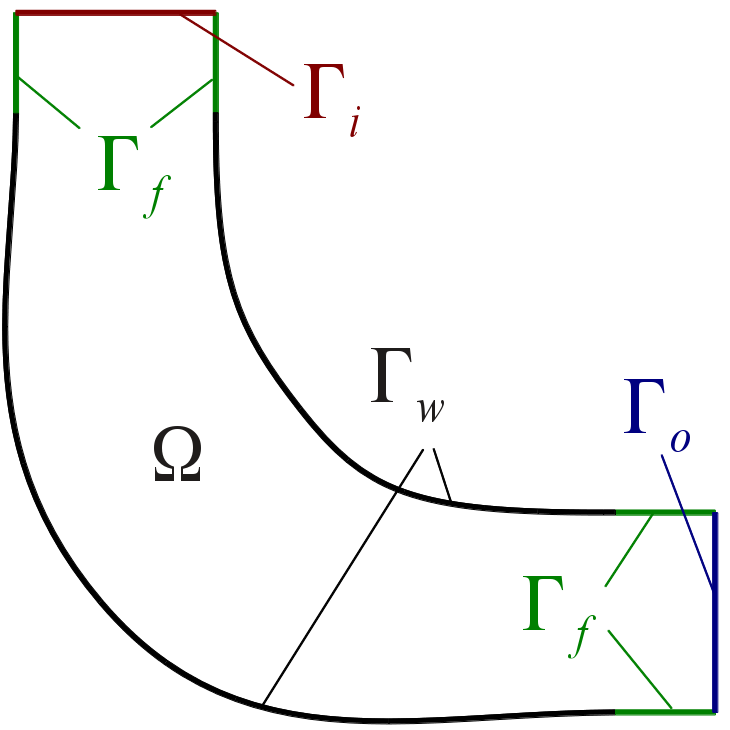
\includegraphics[scale=0.5]{geometrie_skizze_noInterface.png}
    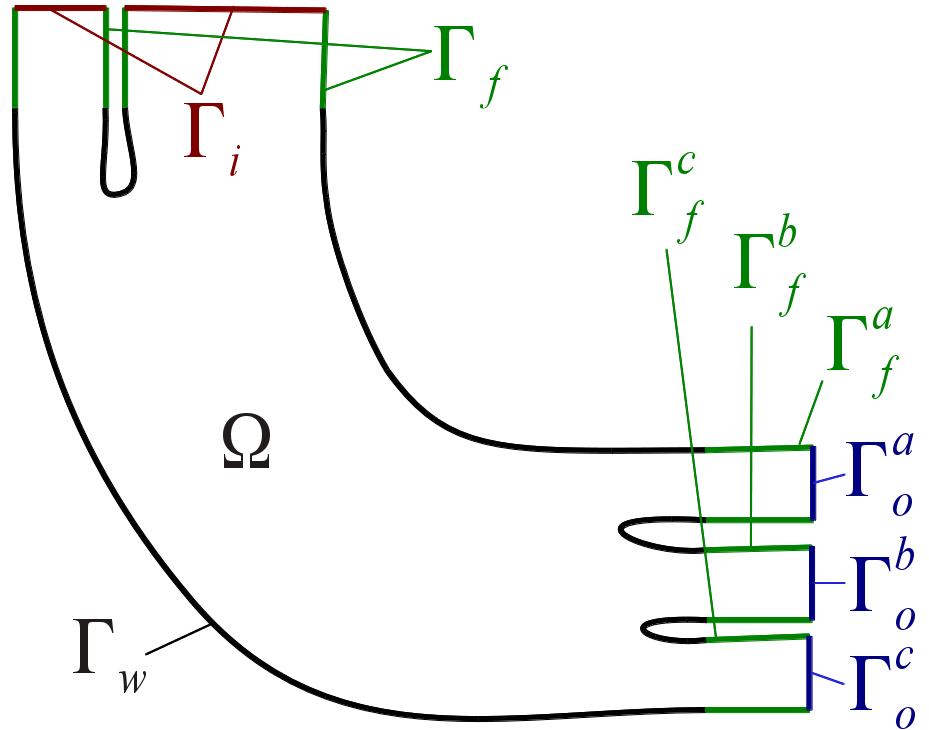
\includegraphics[scale=0.5]{geometrie_skizze_MultOutlet.png}
    \caption{Skizze von $\Om$ mit Bezeichnung der Teile der Oberfläche.}
    \label{Skizze_extrusion}
\end{figure}
The parameters \verb|gnu_plot_visual| and \verb|gnu_plot_visual_i| are used for the graphical representation of the target function values.

If this option is selected, the graphics appear during shape optimization and are stored in the Test Run folder under \verb|Function_values_J1.ps|, \verb|Function_values_J2.ps| and \verb|Function_values_J12.ps|.
\begin{table}[h]
    \centering
    %\begin{tabular}{|p{2.5cm}|p{1.1cm}|p{1.8cm}|p{1cm}|p{4cm}|} %lcrp
    %\hline
    %\cellcolor{light-gray} Parametername & \cellcolor{light-gray} Default-wert & \cellcolor{light-gray} Zulässigkeits-bereich & \cellcolor{light-gray} RLR  & \cellcolor{light-gray} Beschreibung\\
    \begin{tabular}{|p{2.5cm}|p{1cm}|p{1.6cm}|p{0.6cm}|p{1.3cm}|p{4cm}|} %lcrp
        \hline
        \cellcolor{light-gray} Parameter name & \cellcolor{light-gray} Default value & \cellcolor{light-gray} Admissibility & \cellcolor{light-gray} RLR & \cellcolor{light-gray} M23 & \cellcolor{light-gray} Description\\
        \hline
        dp\_J12              &  0.5    & [0,1]    & 0.5   & 0.5 & Weighting parameter $\gamma$ between $\JJ_1$ and $\JJ_2$.\\
        \hline
        dp\_J1              &  1(0)    & $\sum$ dp\_J1 $\in$ [0,1]    & 1(0)   & 3(0.25, 0.25,0.25) & Weighting parameter $\gamma_i$ concerning $\JJ_{1}$.\\
        \hline
        %interface\_fv        &  0      & \{0,1\}  & 0     & 0 & Zielfunktionen auf $\Gamma_i$, $\Gamma_o$ (0) oder Zielfunktionen auf $\overline{\Gamma_i}$, $\overline{\Gamma_o}$ (1).\\
        %\hline
        gnu\_plot\_visual    &  0      & \{0,1\}  & 0     & 0 & Graphic display of the target function values (1). No graphical representation (0).\\
        \hline
        gnu\_plot\_visual\_i &  3      & [1,1000] & 1     & 1 & Update the graphics after ... iterations.\\      
        %\hline
        %sg\_layer            &  0      & [0,100]  & 0     & 1 & 0: Äußerste Randschicht für Formsensitivität; 1,2,...100: innere Randschichten.\\
        \hline
    \end{tabular}
    \caption{Form optimization: Target functionalities}\label{tab:parameter4}
\end{table}

\subsubsection{Target functionalities with multiple outflow ranges}
For illustration we use 3 outflow areas and call them $\Gamma_o^a$, $\Gamma_o^b$, $\Gamma_o^c$. The target functionalities for the even outflow are
\begin{eqnarray}
\JJ_{1}=\JJ_{1}\lvert_{\Gamma_o^a \cup \Gamma_o^b \cup \Gamma_o^c },\quad
\JJ_{1a}=\JJ_{1}\lvert_{\Gamma_o^a },\quad
\JJ_{1b}=\JJ_{1}\lvert_{\Gamma_o^b },\quad
\JJ_{1c}=\JJ_{1}\lvert_{\Gamma_o^c }.
\end{eqnarray}
The mixed objective functional is:
\begin{eqnarray}
\JJ_{12}&=&\left(1-\gamma\right)\left(1-\gamma_a -\gamma_b -\gamma_c\right) \rho_1 \JJ_1 \\
& & + \left(1-\gamma\right) \gamma_a \rho_{1a} \JJ_{1a} + \left(1-\gamma\right) \gamma_b \rho_{1b} \JJ_{1b} + \left(1-\gamma\right) \gamma_c \rho_{1c} \JJ_{1c} \\
& & + \gamma \rho_2 \JJ_2
\end{eqnarray}
with the user-defined weighting parameters $\gamma,\gamma_a,\gamma_b,\gamma_c \in [0,1]$ (\verb|dp_J12|, \verb|dp_J1|) where $\gamma_a + \gamma_b + \gamma_c\le 1$ and the scales $\rho_1$, $\rho_2$, $\rho_{1a}$, $\rho_{1b}$, $\rho_{1c}$, which are calculated as follows if $\gamma < 1$. We define
\begin{eqnarray}
\mu_{uni}= \max \left(\;  
\hat{\gamma_1}\left\Vert\partial \JJ_1 \left(\buu \left( \Om^0 \right) \right) \right\Vert_{L^2\left(\Gamma_w^0\right)} \; , \; 
\hat{\gamma_a}\left\Vert\partial \JJ_{1a} \left(\buu \left( \Om^0 \right) \right) \right\Vert_{L^2\left(\Gamma_w^0\right)} \; , \right.\\
\left.\hat{\gamma_b}\left\Vert\partial \JJ_{1b} \left(\buu \left( \Om^0 \right) \right) \right\Vert_{L^2\left(\Gamma_w^0\right)}\; , \;
\hat{\gamma_c}\left\Vert\partial \JJ_{1c} \left(\buu \left( \Om^0 \right) \right) \right\Vert_{L^2\left(\Gamma_w^0 \; \right)}
\right)
\end{eqnarray}
where $\Omega^0$ and $\Gamma_w^0$ the geometry in the area and at the edge is at the beginning of the shape optimization and
\begin{eqnarray}
\hat{\gamma_1} = \begin{cases} 0 & \mbox{if} \, \gamma_a+\gamma_b+\gamma_c =1,\\
1 & \mbox{if} \, \gamma_a+\gamma_b+\gamma_c <1,
\end{cases}\;
\hat{\gamma_I} = \begin{cases} 0 & \mbox{if} \, \gamma_I = 0,\\
1 & \mbox{if} \, \gamma_I > 0,
\end{cases}
\mbox{with} \, I \in \{ a, b, c \}. \;
%\hat{\gamma_b} = \begin{cases} 0 & \mbox{wenn} \; \gamma_b = 0,\\
%1 & \mbox{wenn} \; \gamma_b > 0,
%\end{cases}
%\hat{\gamma_c} = \begin{cases} 0 & \mbox{wenn} \; \gamma_c = 0,\\
%1 & \mbox{wenn} \; \gamma_c > 0.
%\end{cases}
\end{eqnarray}
The scaling parameters are
\begin{eqnarray}
\rho_k = \frac{\mu_{uni}}{\left\Vert\partial \JJ_k \left(\buu \left( \Om^0 \right) \right) \right\Vert_{L^2\left(\Gamma_w^0\right)}} \; \mbox{with} \; k \in \{1,2,1a,1b,1c\}.
\end{eqnarray}
If $\gamma = 1$, then $\rho_1 = 1$ is set.

\subsection{Geometric restrictions}
The shape optimization is subject to 2 geometrical restrictions:
\begin{itemize}
    \item Installation space restriction: An optimum geometry is sought within a fixed installation space.
    \item Transition restriction: At the transition between the geometry to be shape-optimized and the fixed geometry an edge should be avoided to avoid problems in the flow simulation.
\end{itemize}

\subsubsection{Method 1: Fixing at the transition area}
Shape gradient at the centers of the surfaces adjacent to the fixed geometry set to 0.
\begin{figure}[h]
    \centering
    \begin{minipage}[b]{5 cm}
        Numerical calculation at these locations is not trustworthy. In previous calculations the shape gradient was automatically set to zero on these areas. This is also recommended for further test calculations. The setting is done with the parameter: \verb|uer_fix_faces| (0:do not fix, 1: fix).$ $\\
        $ $\\
        $ $\\
    \end{minipage}
    %    \begin{minipage}[b]{1 cm}
    %     \end{minipage}
    \begin{minipage}[b]{6 cm}
        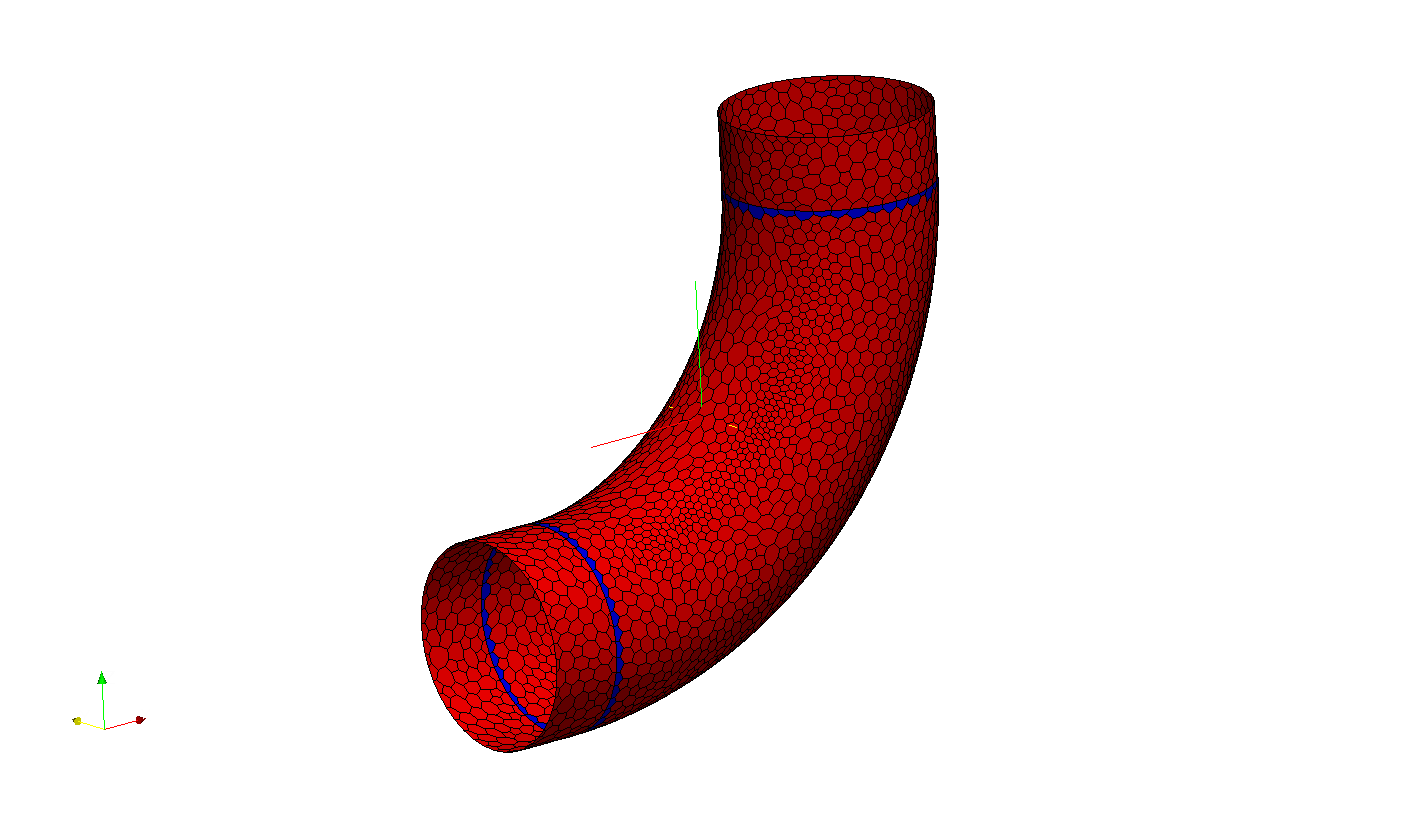
\includegraphics[scale=0.14]{inlet_outlet_fg_fix.png} 
        \caption{BLUE: Faces on which the shape gradient is set to 0 at the center of the surface.}
        \label{uer_model}
    \end{minipage}
\end{figure}

\subsubsection{Method 2: Use of objective functionals for installation space and transition restrictions}
To take these restrictions into account in shape optimization, the previously used objective function $\mathcal{J}_12$ is extended to
\begin{equation}
\nonumber  \JJ_{12}^{\alpha,\varphi}\left( \buu \left( \Om \right) \right)=\JJ_{12}\left( \buu \left( \Om \right) \right)+ \alpha \LL\left(\Om\right) + \varphi \LL_F\left(\Om\right)
\end{equation}
with $\LL\left(\Om\right)=\int_\Om \ell\left( x \right)$, $\LL_{F}\left(\Om\right)= \int_{\Om} (d(x,K_F))^2$, the weighting parameters $\alpha\ge 0$ (\verb|installation_weighting|), $\varphi\ge 0$ (\verb|fixed_weighting|) and the distance function $d(x,K_F) = c_1\min_{y\in K_F} |x - y|$. In the case of the barrier method, $l(x) = |\log d(x,K^c)|$ and in the case of the penalty method, $l(x) = c_2(d(x,K))^\beta$, with $\beta > 0$ (\verb|bauraum_straf_potenz|). The scaling factors $c_1$, $c_2$ are discussed in section 3.7.3. The geometry $K$ denotes the installation space geometry, $K^c = \mathbb{R}^n\backslash K$ and the geometry $K_F$ denotes the permissible range of the geometry in the transition between the fixed parts and the parts to be optimized. The \verb|bauraum_restriction| parameter specifies whether and/or which method is to be used for dealing with the installation space restriction. The parameters \texttt{OuterLoopCycleNr} (Table 8) and \verb|bauraum_modification_scale| can be used to increase (in case of the penalty method) or decrease (in case of the barrier method) the installation space weighting $\alpha$ during the shape optimization process.
\begin{figure}[h]
    \centering
    \begin{minipage}[b]{5 cm}
        Within the area defined by the distance to the fixed geometry (\verb|uer_bereich|) the transition restriction is applied. The user can control the restriction geometry with the parameters: \verb|uer_pow| (degree of power function of the nonlinear portion), \verb|uer_nonlinear|, and \verb|uer_linear| (see Fig. 3.3).
        $ $\\
    \end{minipage}
    \begin{minipage}[b]{0.5 cm}
        $ $\\
    \end{minipage}
    \begin{minipage}[b]{6 cm}
        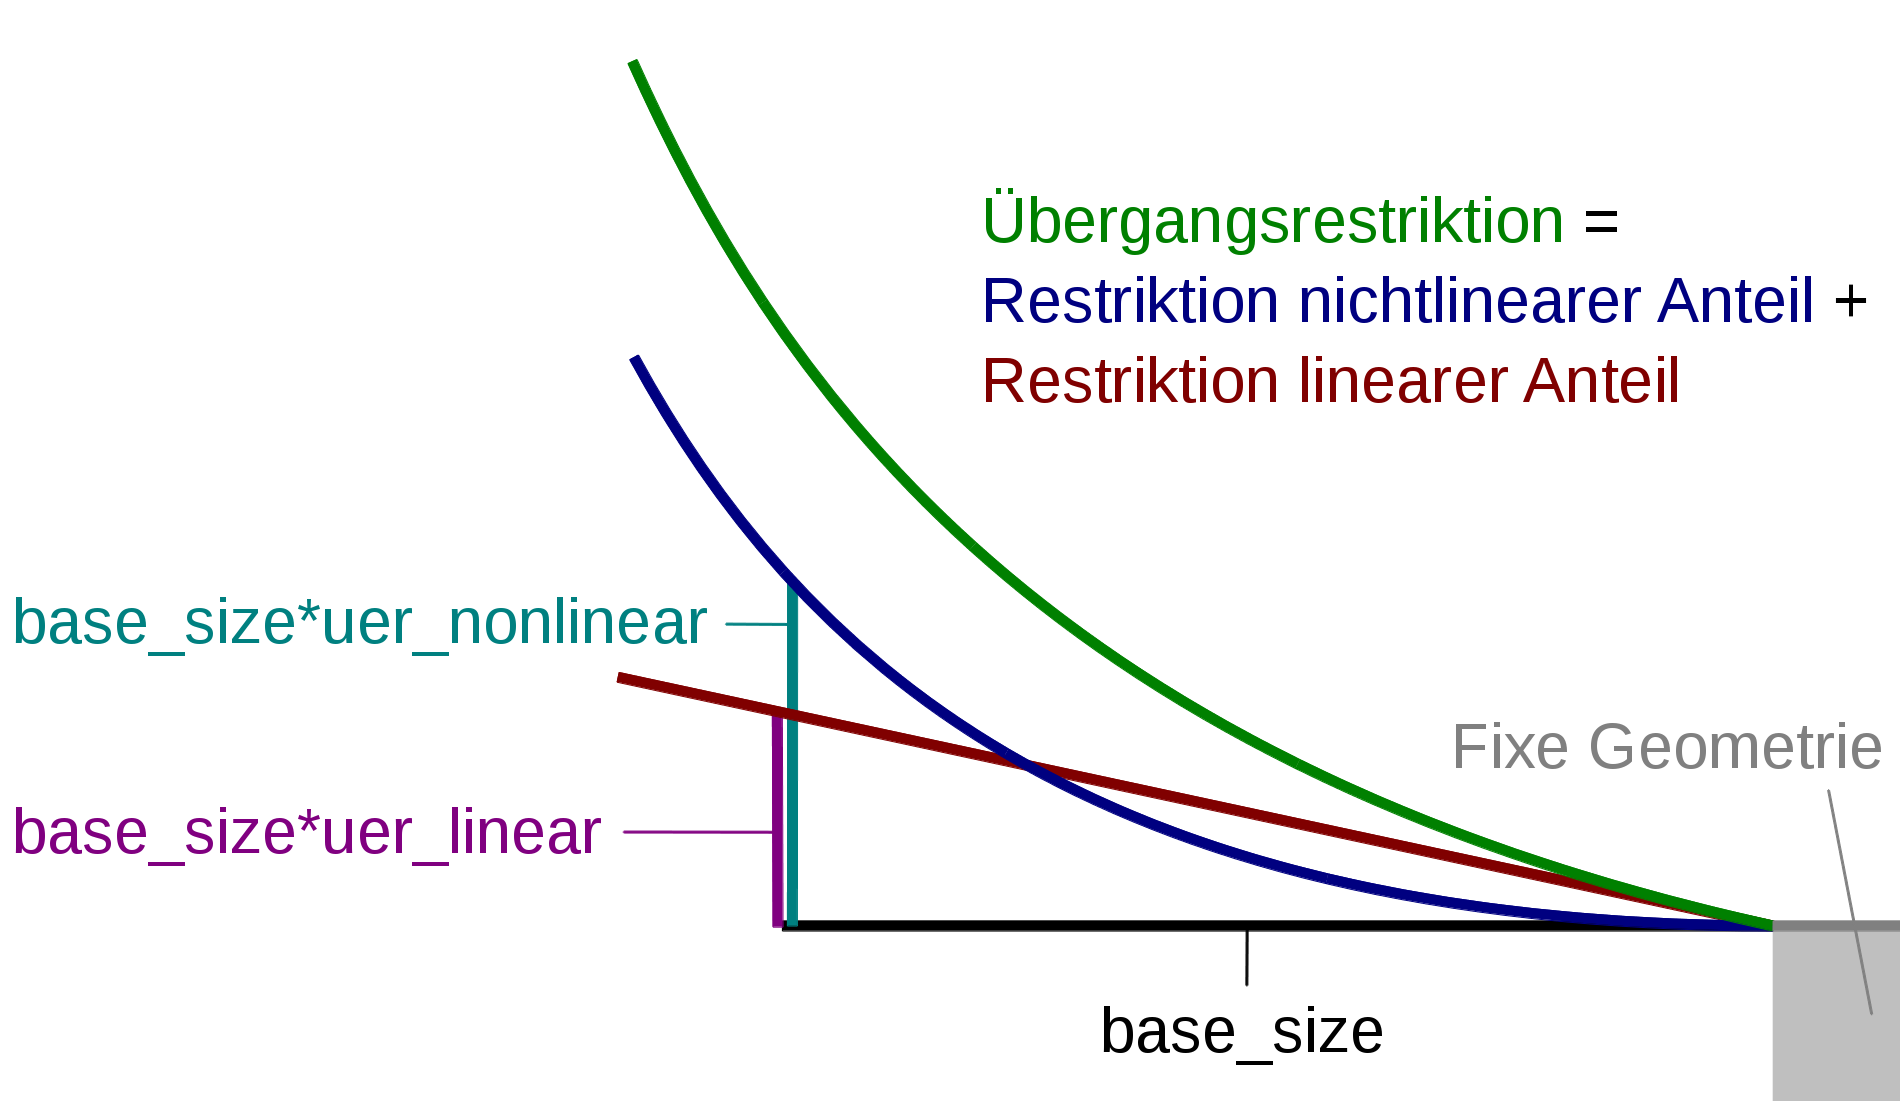
\includegraphics[scale=0.4]{uer_funk2.png}
        \caption{Transition geometry.} 
        \label{uer_model}
    \end{minipage}
\end{figure}
%
\begin{figure}[htbp]
    \centering
    %    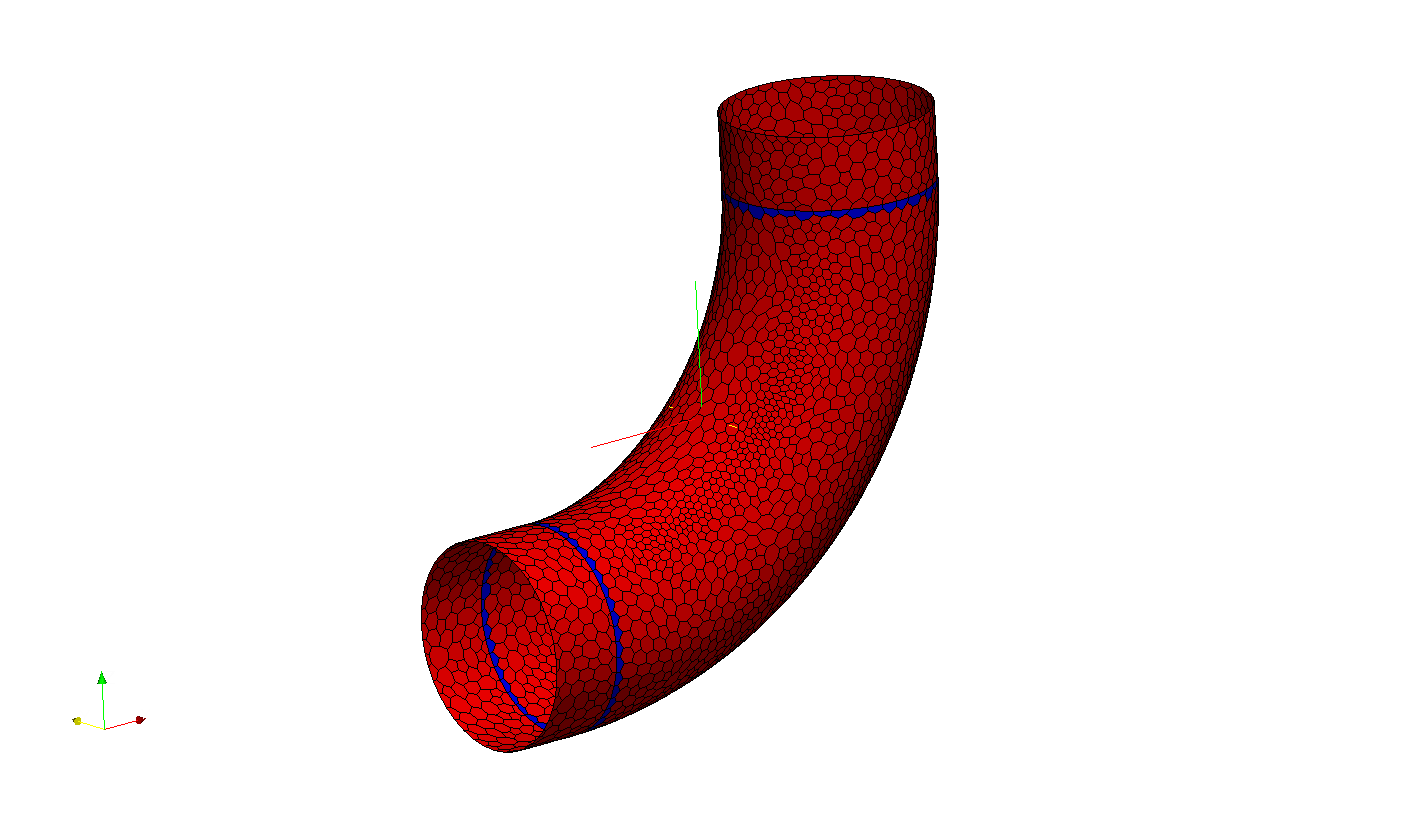
\includegraphics[scale=0.13]{inlet_outlet_fg_fix.png} 
    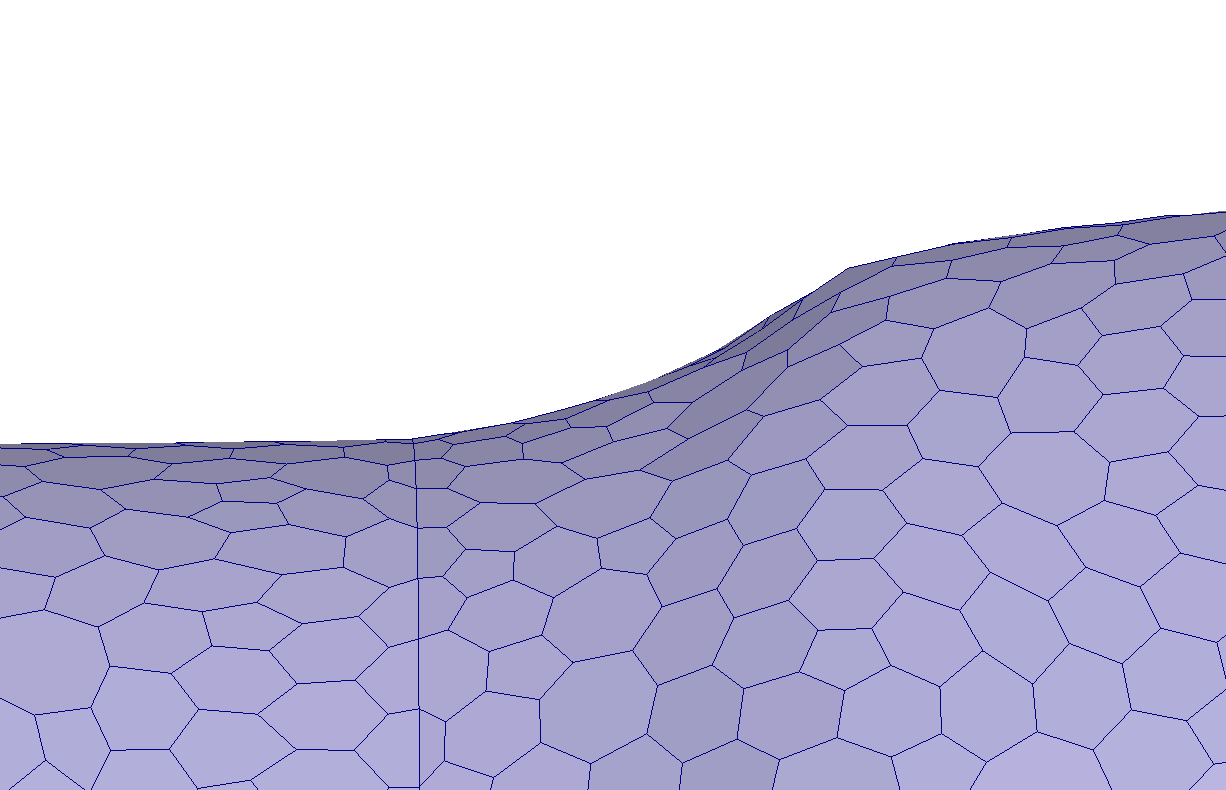
\includegraphics[scale=0.1]{restriktion1.png} 
    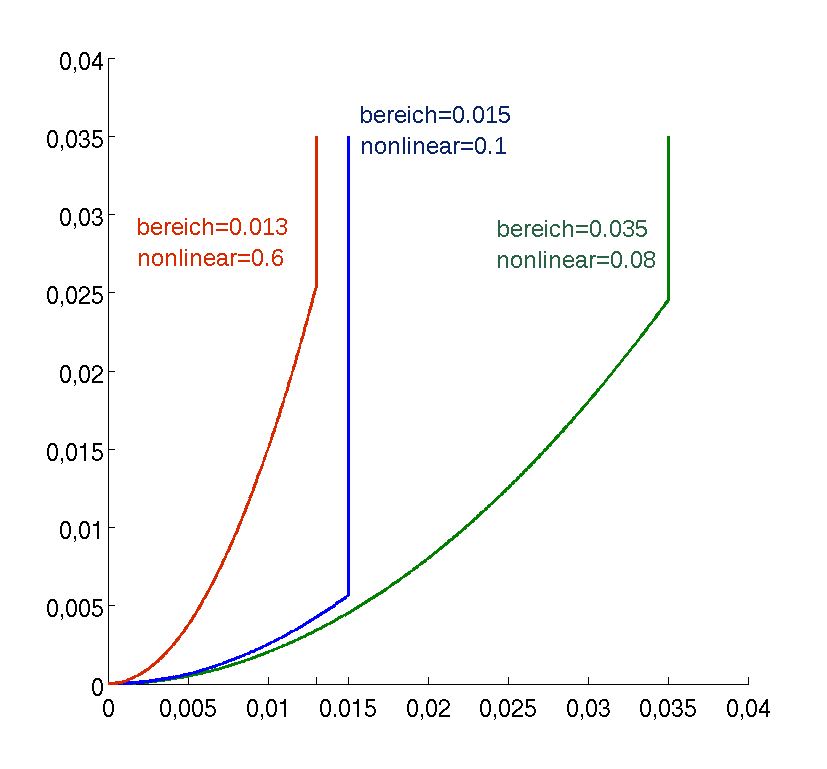
\includegraphics[scale=0.25]{uer_bereich_nonlinear.png} 
    %    \includegraphics[scale=0.1]{Rohr1a_J0_v2.png} 
    \caption{Left: Geometry at the transition. Right: different transition restrictions.} 
    \label{uer_3kurven}
\end{figure}
Figure \ref{uer_3kurven} shows transition curves for three different parameter settings. In order to avoid strong curvatures of the geometry, the variant in green color is recommended.

\subsubsection{Heuristic scaling of the target functionals in geometrical restrictions}
To achieve equal orders of magnitude of geometric objective functionals and physical objective functionals, we use a scale $c_1$ of the spatial coordinates and a scale $c_2$ of the function $l(d)$ using the starting geometry $\Omega^0$. In the case of the \textbf{penalty method}, the parameters $c_1$ and $c_2$ are chosen so that the equations
\begin{eqnarray}
\int_{\Sigma\left(d_{min}\right)}\int_0^{c_1 d_{max}} c_2 d^{\beta} \text{d}d &=& \JJ_{12}\left( \buu \left( \Om^0 \right) \right), \\
c_2\left(c_1 d_{max}\right)^\beta &=& \lVert \DD \JJ_{12}^\alpha \left( \Om^{0}  \right) \rVert_{L^\infty \left(\Gamma_w^0\right)}
\end{eqnarray}
where $d_{\min}$ and $d_{\max}$ are to be specified by selecting the \texttt{dminDS} and \texttt{dmaxDS} parameters for the installation space restriction (or analog \texttt{dminIF} and \texttt{dmaxIF} for the transition restriction).
\begin{figure}[htbp]
    \centering
    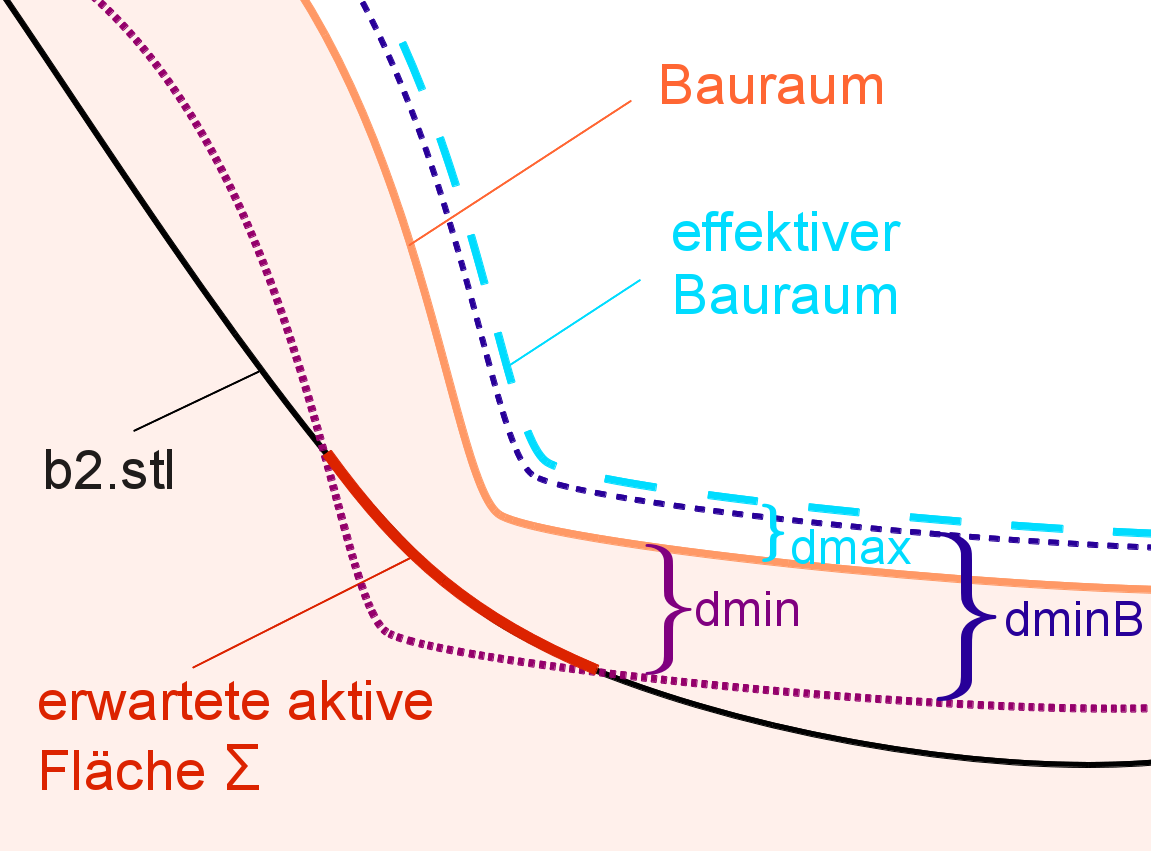
\includegraphics[scale=0.45]{bauraum_parameter1deutsch.png} \quad
    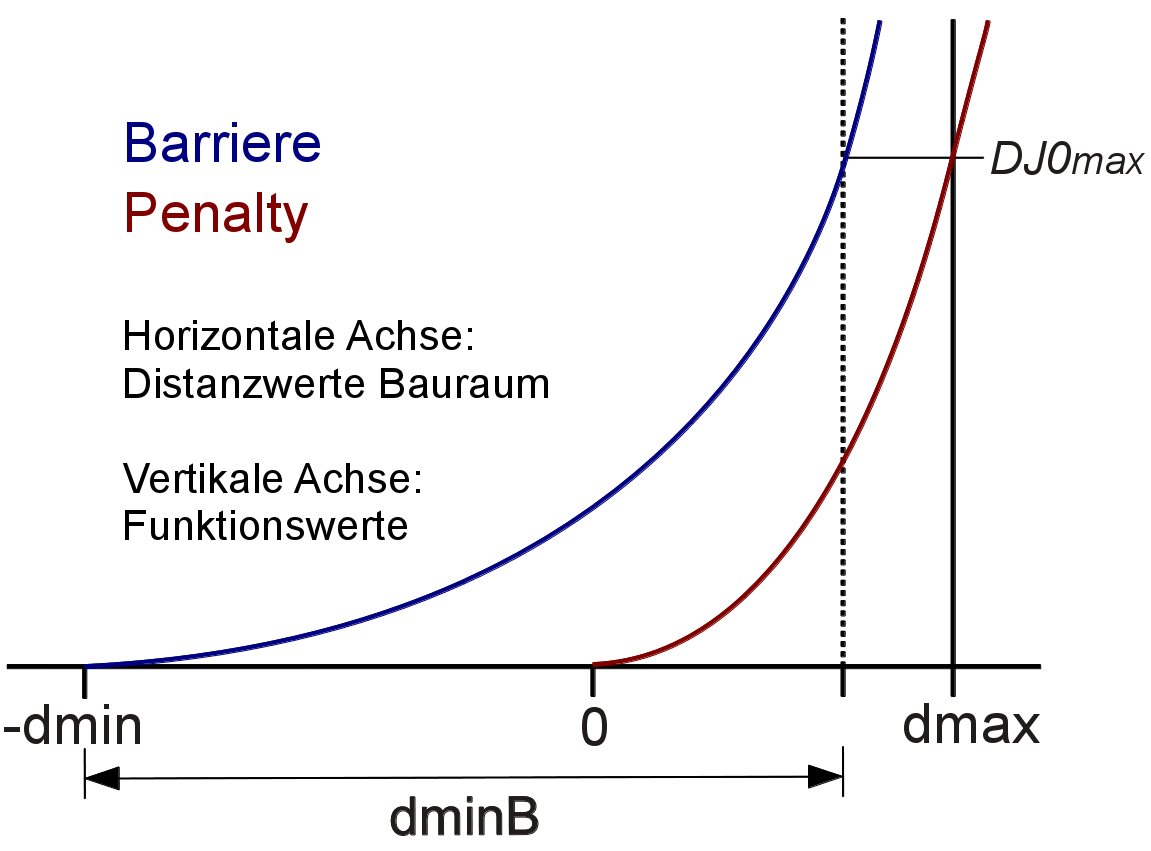
\includegraphics[scale=0.45]{bauraum_parameter2.png} 
    \caption{Left: Sketch installation space. Right: Functions: Penalty, Barrier.} 
    \label{fig:bauraum_parameter}
\end{figure}
In the case of the \textbf{barrier method}, an effective installation space can be selected instead of the geometric installation space (\texttt{bds.stl}). In this case the installation space is increased by the length \texttt{dmaxDS} (unit in meters). If this parameter is set to 0, the effective installation space is equal to the geometric installation space. The setting of \texttt{dmaxDS} greater than 0 is intended in particular for those cases where the start geometry lies outside the geometric installation space. The scaling variables $c_1$ and $c_2$ are selected so that the equations 
\begin{eqnarray}
\int_{\Sigma\left(d_{min}\right)}\int_0^{c_1 d_{minB}} c_2 d^{\beta} \text{d}d &=& \JJ_{12}\left( \buu \left( \Om^0 \right) \right), \\
c_2\left(c_1 d_{minB}\right)^\beta &=& \lVert \DD \JJ_{12}^\alpha \left( \Om^{0}  \right) \rVert_{L^\infty \left(\Gamma_w^0\right)}
\end{eqnarray}
are fulfilled, where $d_{min}$ and $d_{minB}$ are to be specified by selecting the \textbf{dminDS} and \textbf{dminBDS} parameters (see figure \ref{fig:bauraum_parameter}).

\subsubsection{Method 3: Damping in the transition area}
Damping of the shape gradient in the transition area.
\begin{figure}[htbp]
    \centering
    %    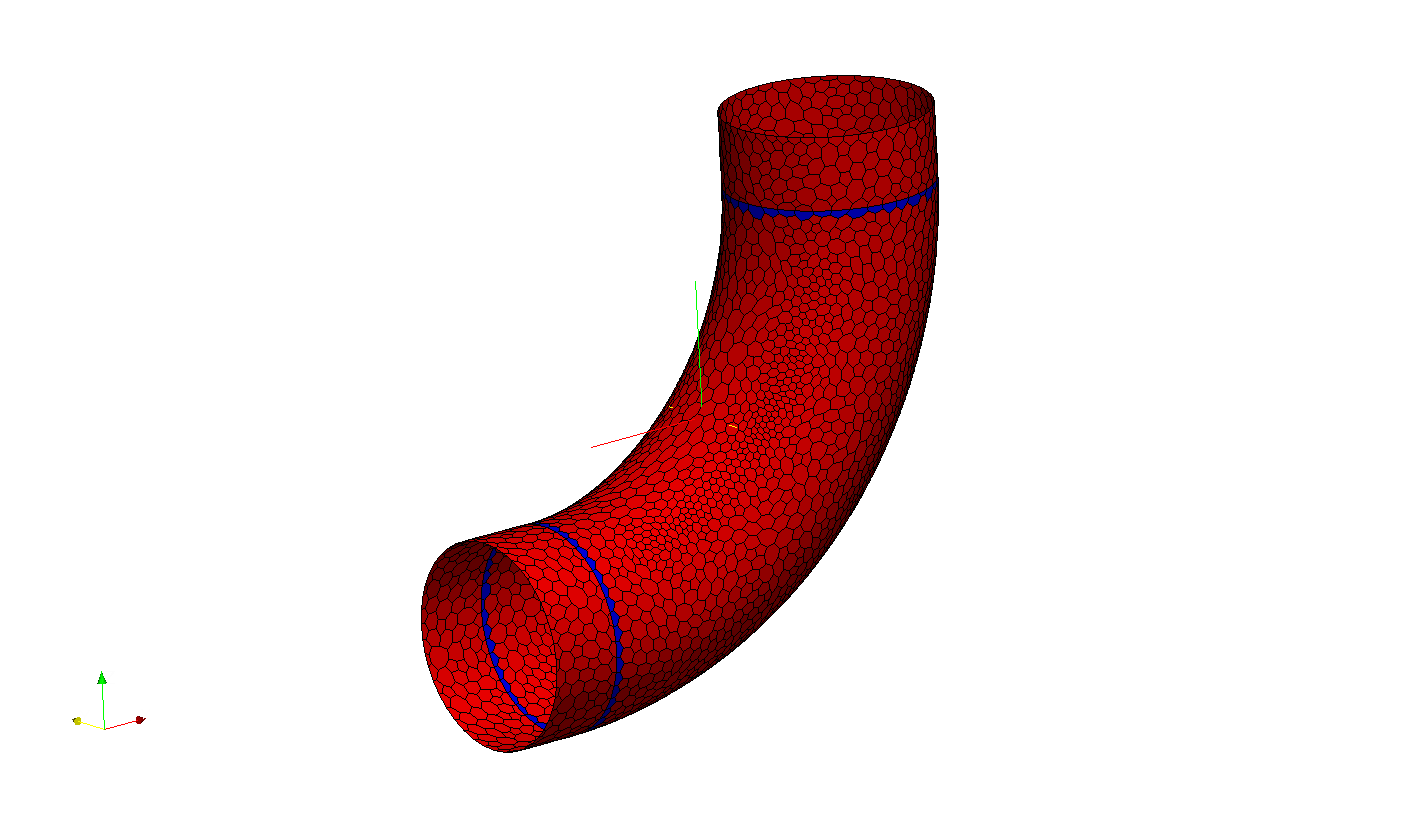
\includegraphics[scale=0.13]{inlet_outlet_fg_fix.png} 
    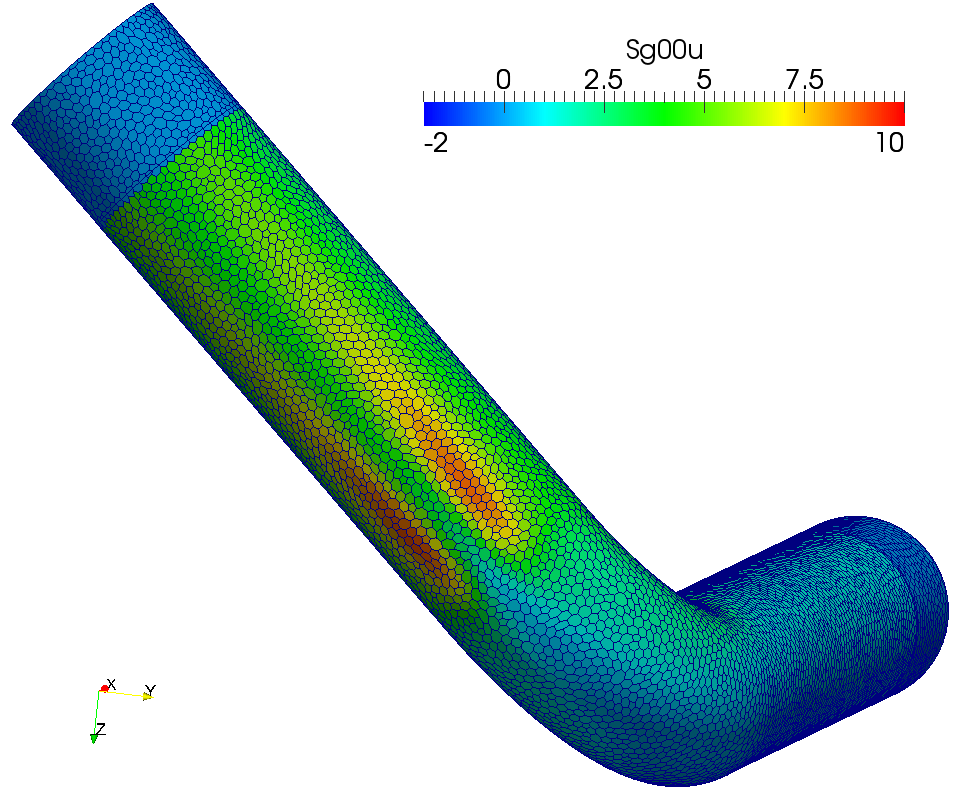
\includegraphics[scale=0.16]{Rohr3_damp0.png} 
    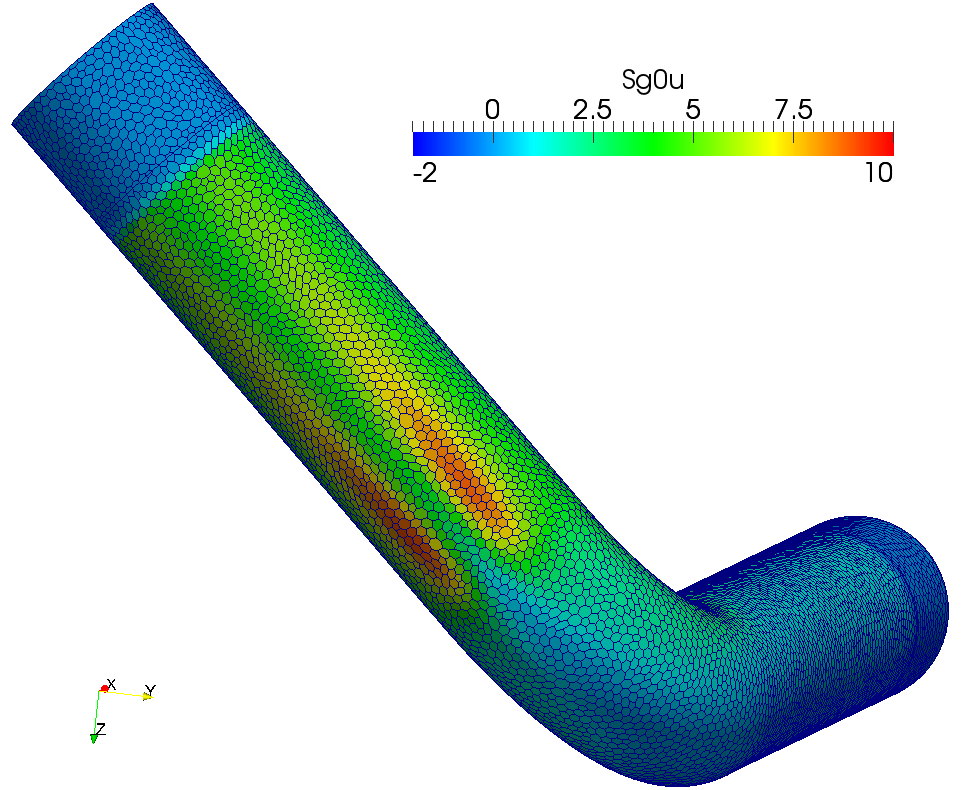
\includegraphics[scale=0.16]{Rohr3_damp1.png} 
    \caption{Left: Tube 3 without damping. Right: Tube 3 with damping.} 
\end{figure}
Properties:
\begin{itemize}
    \item - Unfavorable with inadmissible start geometry.
    \item - Undesirable effects in the transition from attenuated to undamped areas.
    \item + Easy user handling, as no additional parameter is required.
\end{itemize}
\begin{figure}[htbp]
    \centering
    %    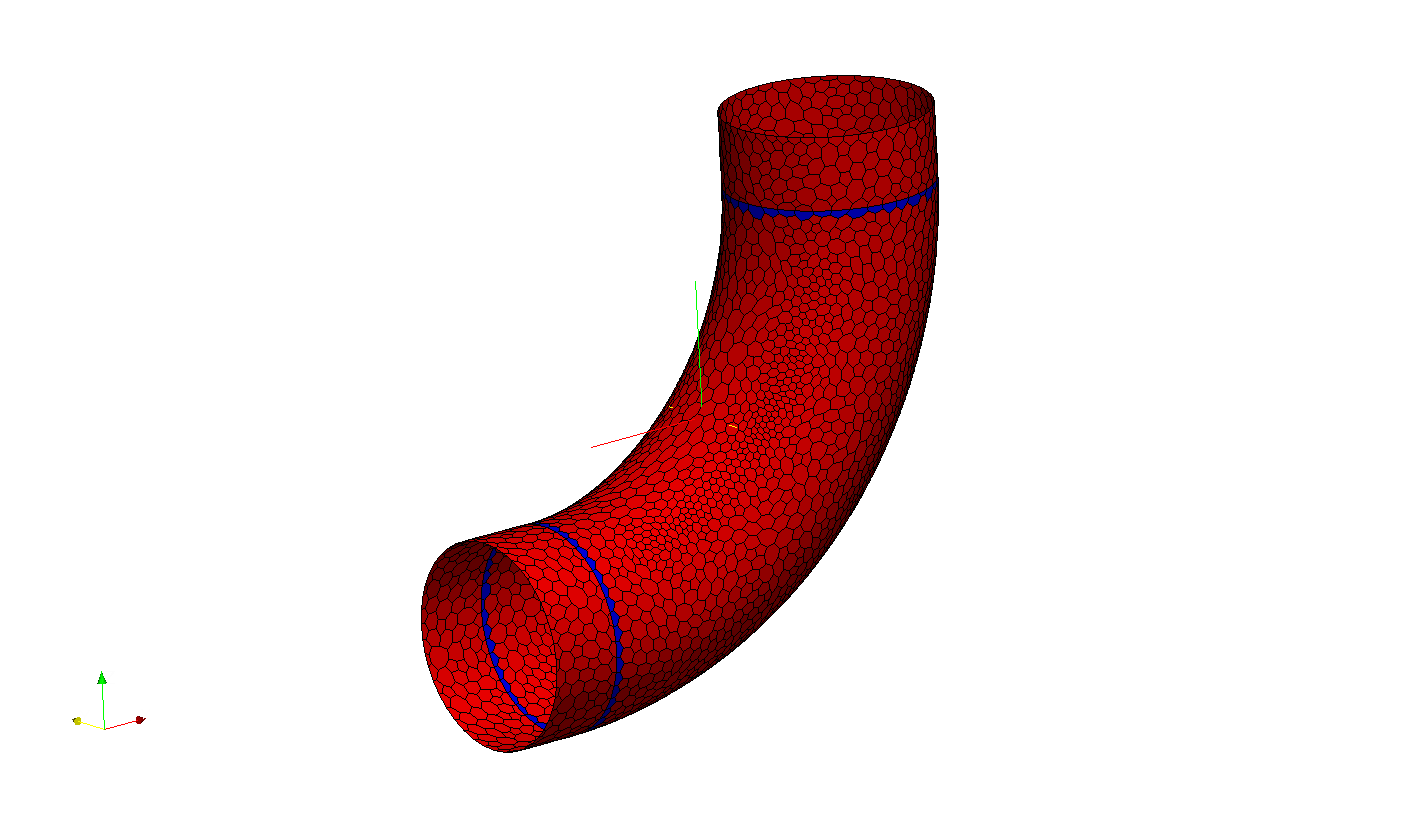
\includegraphics[scale=0.13]{inlet_outlet_fg_fix.png} 
    %   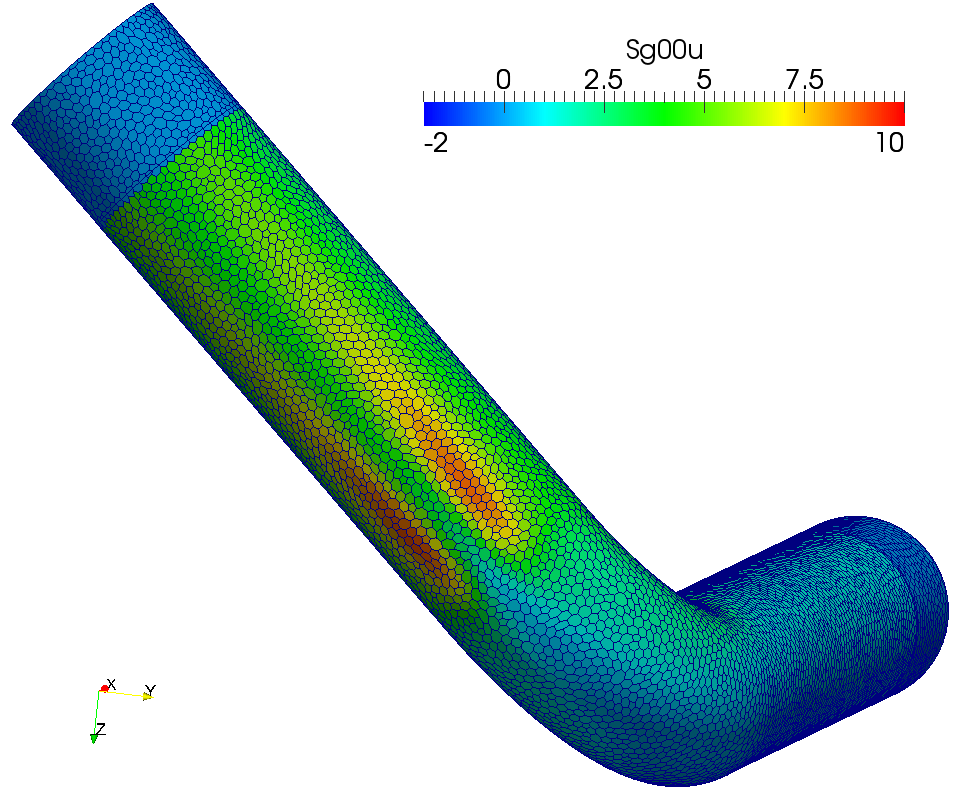
\includegraphics[scale=0.1]{Rohr3_damp0.png} 
    %    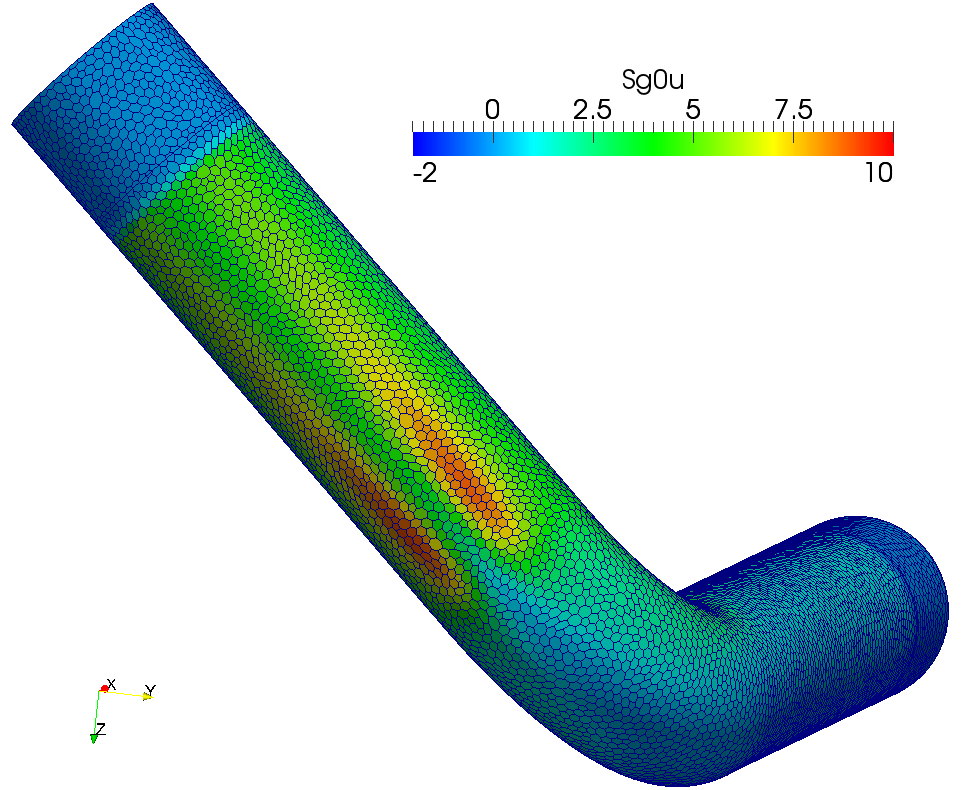
\includegraphics[scale=0.1]{Rohr3_damp1.png}\\
    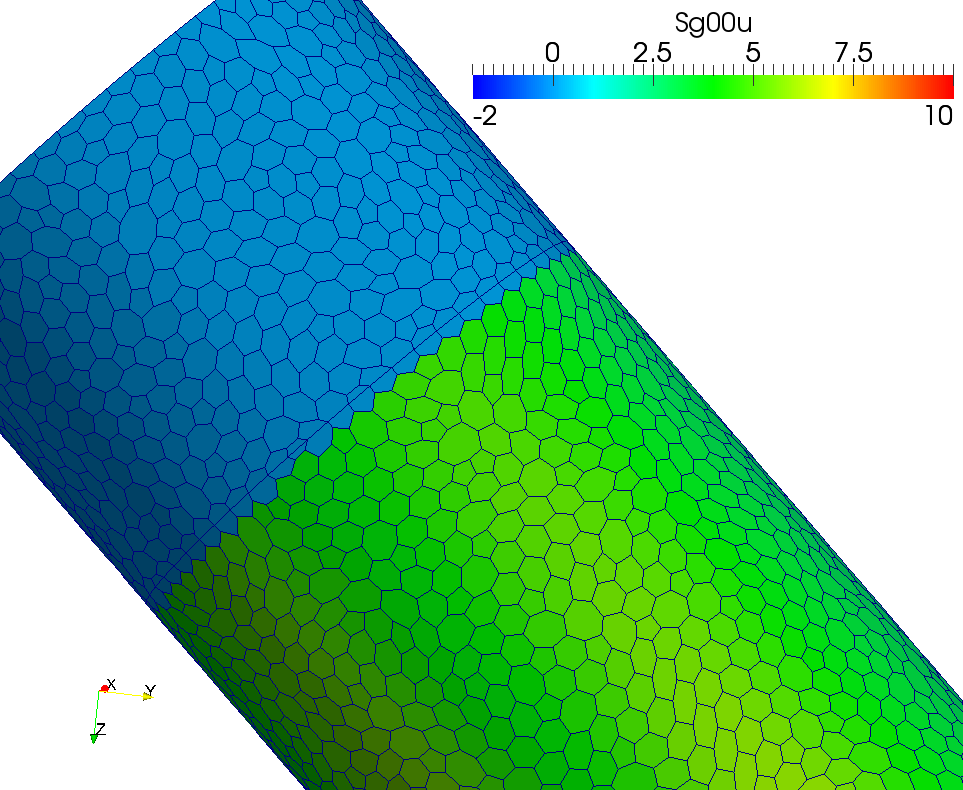
\includegraphics[scale=0.085]{Rohr3_damp_0b.png} $ $
    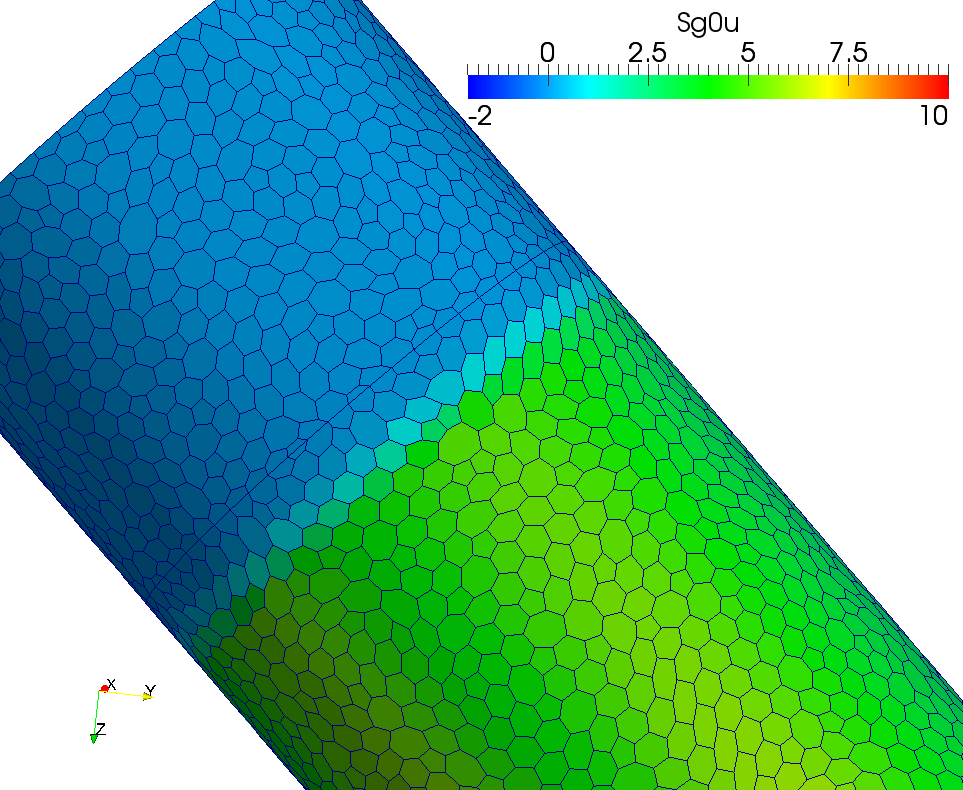
\includegraphics[scale=0.085]{Rohr3_damp_0a.png} $ $
    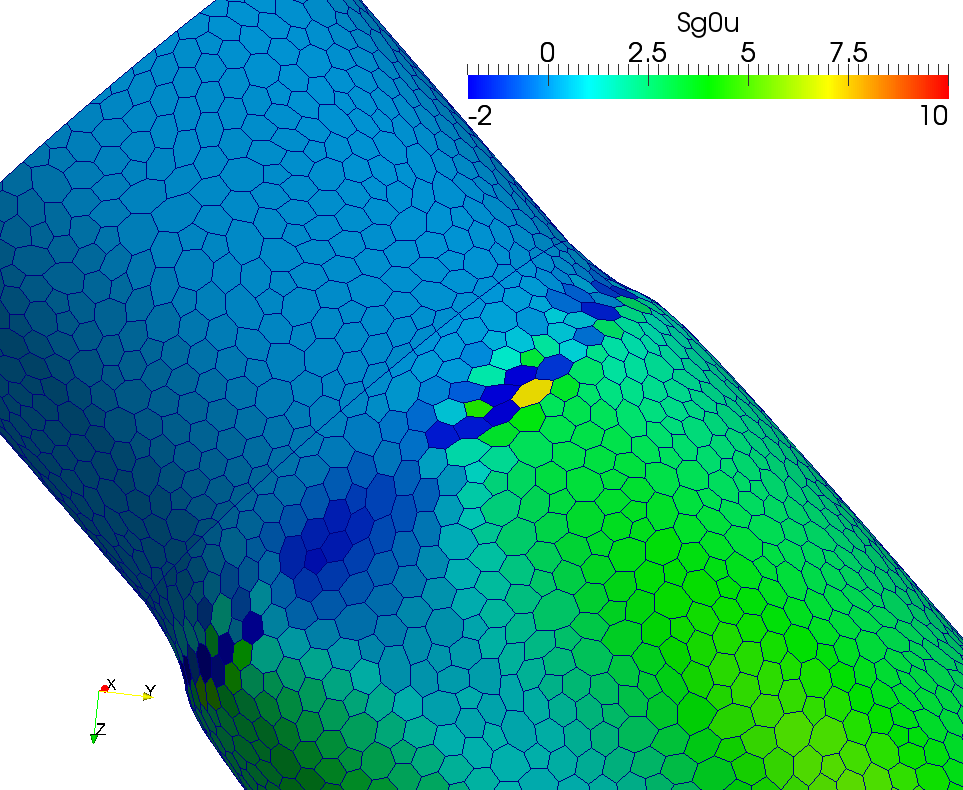
\includegraphics[scale=0.085]{Rohr3_damp40.png}
    %    \includegraphics[scale=0.1]{Rohr1a_J0_v2.png} 
    \caption{Detailed view: left: without damping, middle: with damping, right: damped shape gradient after 40 iterations.}
\end{figure}

\subsubsection{Method 4: Smoothing the shape gradient}
Solve the Laplace-Beltrami equation with boundary conditions equal to 0 on the transition curve.
\begin{figure}[htbp]
    \centering
    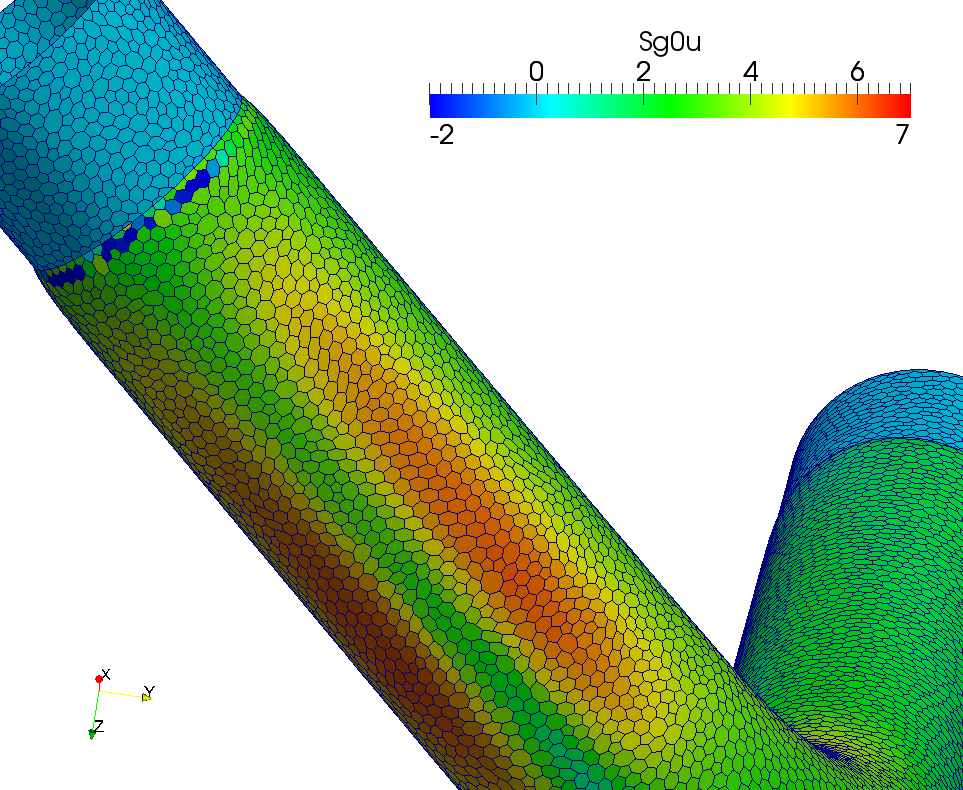
\includegraphics[scale=0.12]{Rohr3_lb0.png} 
    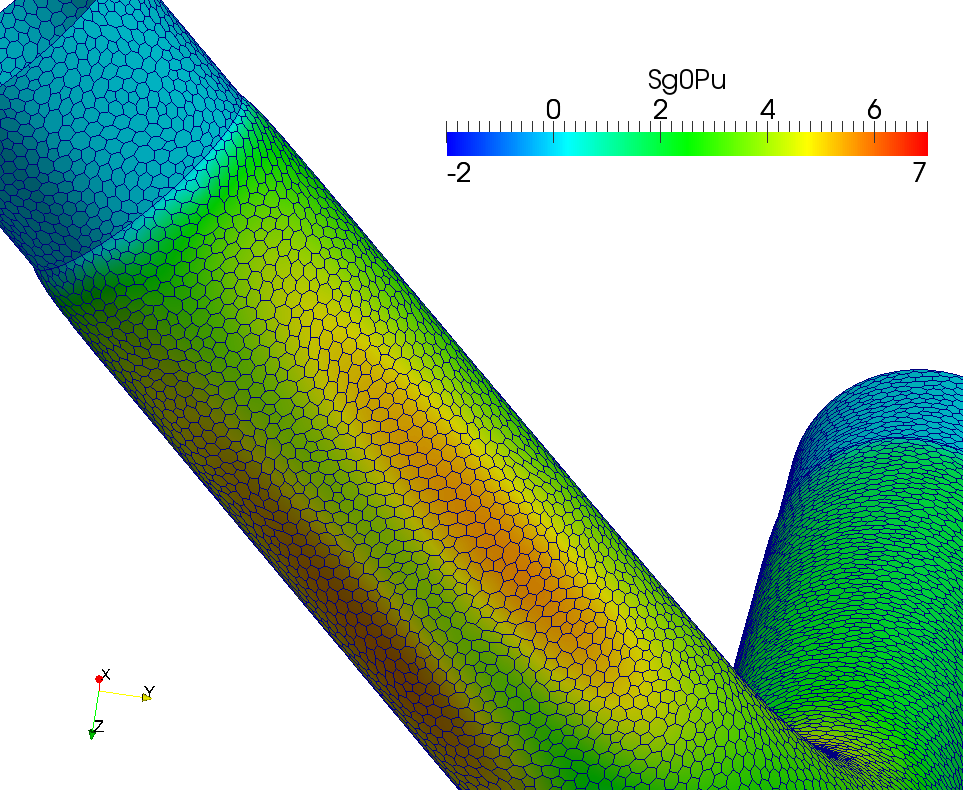
\includegraphics[scale=0.12]{Rohr3_lb1.png} 
    \caption{Rohr 3: links: ohne LB-Glättung, rechts: mit LB-Glättung.} 
\end{figure}
$ $\\
\begin{eqnarray}
\label{LB1} -\varepsilon \Delta_\Gamma w + w &=& -g_{\JJ_{12}}  \qquad \mbox{auf}\quad \Gamma\\
w &=& 0 \qquad \qquad \, \mbox{auf}\quad \partial \Gamma
\end{eqnarray}
$ $\\
The parameter $\varepsilon$ in equation \eqref{LB1} corresponds to the parameter \texttt{scaleLB} in table \ref{tab:parameter8}. If no Laplace-Beltrami smoothing is to be performed, this parameter must be set to 0. Experience shows that the parameter should be selected in the range [1e-6, 1e-3]. Smoothing becomes stronger the larger the parameter is selected.

\begin{table}[h]
    \centering
    \begin{tabular}{|l|p{1cm}|p{1.2cm}|p{0.7cm}|p{0.7cm}|p{5.7cm}|} %lcrp
        \hline
        \cellcolor{light-gray} Parameter name & \cellcolor{light-gray} Default value & \cellcolor{light-gray} Admissibility & \cellcolor{light-gray} RLR & \cellcolor{light-gray} M23 & \cellcolor{light-gray} Description \\
        \hline
        uer\_bereich                   &  0.01  &  [0,100]   & 0.015 & 0.35 & Transition restriction: Range in m.\\
        \hline
        uer\_nonlinear                 &  0.2   &  [0,100]   & 0.6   & 0.3 & Übergang.: <<1: flache, >>1:steile Kurve.\\
        \hline
        uer\_linear                    &   0    &  [0,100]   & 0     & 10 & Transition: <<1: flat, >>1:steep curve.\\
        \hline
        uer\_pow                       &  2     &  [0,10]    & 2     & 2 & Transition: Potency of the transition fact.\\
        \hline
        bauraum\_restriktion           &  1     &  \{0,1,2\} &  2    & 0 & 0:without installation space, 1:barrier, 2:penalty.\\
        \hline
        %bauraum\_gewichtung            &  1     &  [0,1e22]  &  1    & 1 & Gewichtung $\alpha$ für Bauraumrestriktion.\\
        %\hline
        bauraum\_straf\_potenz        &  2     &  [1,3]     &  2    & 2 & Potency $\beta$ in penalty proceedings.\\
        \hline
        fix\_gewichtung                &  1     &  [0,100]   &  1    & 1 & Weighting $\varphi$ for transition restriction.\\
        \hline
        uer\_fix\_faces                &  1     &  \{0,1\}    & 1     & 1 & Transition restriction: Use method 1: 0:no, 1:yes.\\
        \hline
        scaleShapeGradientFix          &  1     &  \{0,1\}    & 1     & 0 & Transition restriction: Use method 3: 0:no, 1:yes.\\
        \hline
        scaleLB                        &  1e-5  &  [0,1]      & 5e-5  & 1e-3 & Transition restriction: Method 4 smoothing parameters: 0 no smoothing, 1 strong smoothing.\\
        \hline
    \end{tabular}
    \caption{Geometric restrictions 1.}\label{tab:parameter8}
    $ $\\
    %\end{table}
    %
    %\begin{table}[h]
    %\centering
    \begin{tabular}{|p{2.5cm}|p{3.7cm}|p{1cm}|l|} %lcrp
        \hline
        \cellcolor{light-gray} Parameter name & \cellcolor{light-gray} Default value & \cellcolor{light-gray} Admissibility  & \cellcolor{light-gray} Description \\
        \hline
        dminIF, dmaxIF   &  1e-2, 5e-3  &  [0,10]       & Transition Restriction: Scaling.\\
        \hline
        dminDS, dminDS   &  1e-2, 5e-3  &  [0,10]      & Installation space restricted: Scaling.\\
        \hline
        dminBDS          &  (dminDS+dmaxDS)*0.8  &  [0,10]      & Installation space restricted: Scaling. \\
        \hline
    \end{tabular}
    \caption{Geometric restrictions 2 (detail).}\label{tab:parameter8}
    %\end{table}
    %
    $ $\\
    %\begin{table}[h]
    %\centering
    \begin{tabular}{|p{1.6cm}|p{1.2cm}|p{1cm}|p{7.6cm}|} %lcrp
        \hline
        \cellcolor{light-gray} Parameter name & \cellcolor{light-gray} Default value & \cellcolor{light-gray} Admissibility  & \cellcolor{light-gray} Description \\
        \hline
        restart\_opt      &  0  &  \{0,1\}       & Use initial geometry \texttt{wall0.stl} for geometry change: 0:no, 1:yes. \\
        \hline
        damp           &  3(0 0 0)  &  [0,1e20]      & Damping parameters ($\rho_2$, $\rho_1$, $\rho_{1a}$, $\rho_{1b}$, $\rho_{1c}$), to be optionally specified based on the entries in Test Run\_Info.txt.\\
        \hline
    \end{tabular}
    \caption{Optional restart parameters.}\label{tab:parameter9}
\end{table}
%
\newpage 
$ $\\
\newpage

\subsection{Topology optimization}
If topology optimization is to be performed, the parameter \texttt{topOpt} must be set to 1. The adapted impulse equation of the flow in a porous medium is:
%The adapted momentum equation for a porous medium:
\begin{equation}
\nabla \cdot \left(\buu \buu^{T} \right) -\nu \Delta \buu + \nabla p \, \, \textcolor{blue}{ + \, P_V \buu + P_I \left| \buu \right| \buu } = \bzz,
\end{equation}
The maximum values for $P_V$ and $P_I$ must be specified by the parameters \texttt{porosityV} and \texttt{porosityI}. These values are multiplied by the parameter \texttt{startPOR} to determine the initial porosity.

\begin{minipage}[b]{9.2 cm}
    It seems to be numerically necessary to define limits $\TT_{upper}$ (\textbf{thresholdTOPupper}) and $\TT_{lower}$ (\textbf{thresholdTOPlower}) at which the porosity is increased or decreased. 
    Theoretical determination would be $\TT_{upper}=\TT_{lower}=0$.\\\
    Separate scaling of the values greater than $\TT_{upper}$ and the smaller $\TT_{lower}$ leads to $\overline{\alpha}$ (see right figure).
    If this scaling is desired, set \textbf{boundPOR} to 1.
\end{minipage}
\begin{minipage}[b]{3.5 cm}
    %\begin{figure}[htbp]
    \centering
    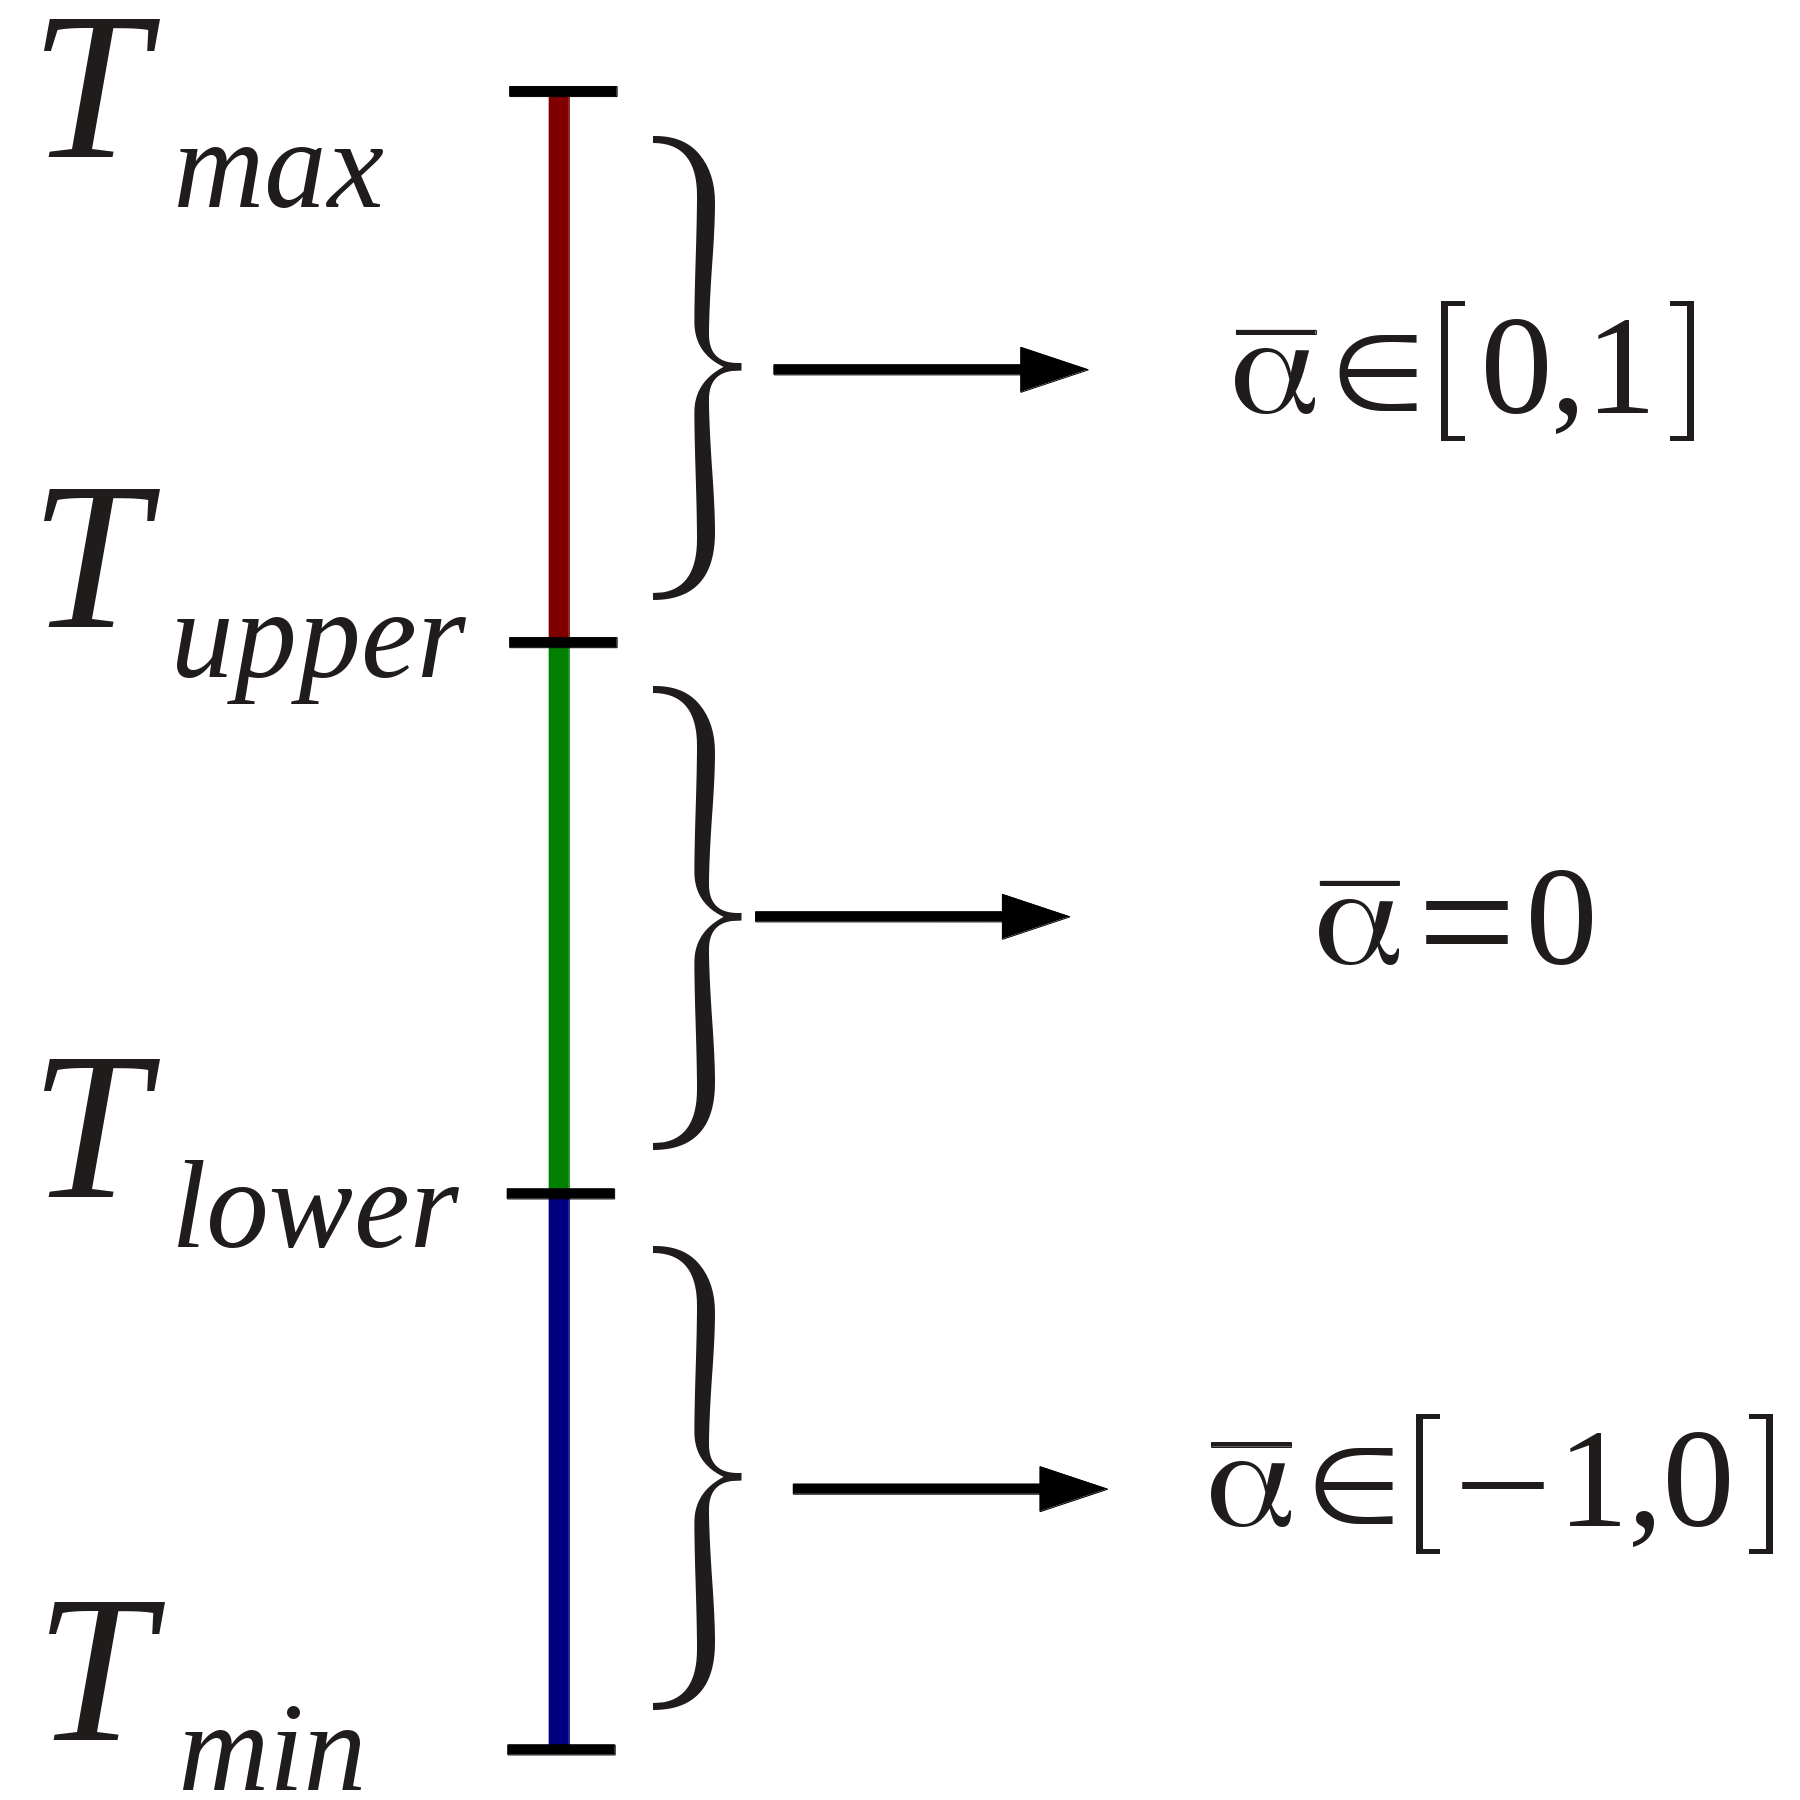
\includegraphics[scale=0.16]{TOPscale.png}
    %\caption{Computation of $\overline{\alpha}$.} 
    %  \label{TopoScale}
    %\end{figure}
    %aaa
\end{minipage}
\begin{table}[h]
    \centering
    \begin{tabular}{|p{2.7cm}|p{1cm}|p{1.2cm}|p{0.9cm}|p{4.7cm}|} %lcrp
        \hline
        \cellcolor{light-gray} Parameter name & \cellcolor{light-gray} Default value & \cellcolor{light-gray} Admissibility  & \cellcolor{light-gray} B135 & \cellcolor{light-gray} Description \\
        \hline
        topOpt                  &  0  &  \{0,1\}          &  1   & 0:shape optimization, 1: topology optimization.\\
        \hline
        startPOR                &  0  &  [0,1]            &  0.1 & Scaling of the starting porosity.\\
        \hline
        porosityI               &  0  &  [0,1e6]          &  0   & Porous Inertial Resistence (maximaler Wert).\\
        \hline 
        porosityV               &  0  &  [0,1e6]          &  150 & Porous Viscous Resistence (maximaler Wert).\\
        \hline
        boundPOR                &  1  &  \{0,1\}          &  1   & Use of the scaling technique.\\
        \hline
        thresholdTOPupper       &  2  &  [0,10]           &-1e-4 & Upper limit value for porosity update.\\
        \hline
        thresholdTOPlower       &  1  &  \{0,1,2\}        &-0.05 & Lower limit for porosity update.\\
        \hline
    \end{tabular}
    \caption{Topology optimization.}\label{tab:parameter10a}
\end{table}
$ $\\
\newpage
\subsection{Extraction of the topology-optimized geometry}
The extracted geometry can be based on the porosity or the topological gradient (\verb|grad_por|). With the parameter \texttt{extractFolder} the folder number in which the desired data set is located has to be specified. Instead of the original data $T_\sigma$ can be used:
\begin{figure}[htbp]
    \centering
    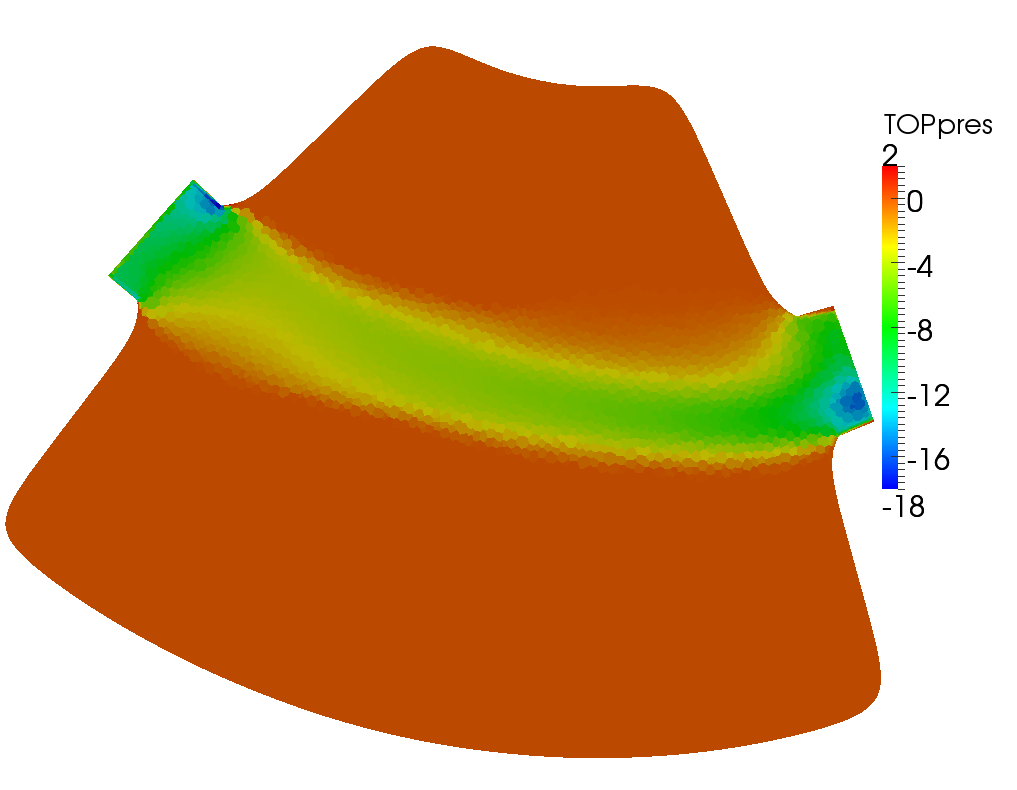
\includegraphics[scale=0.1]{TS2e5top2.png}
    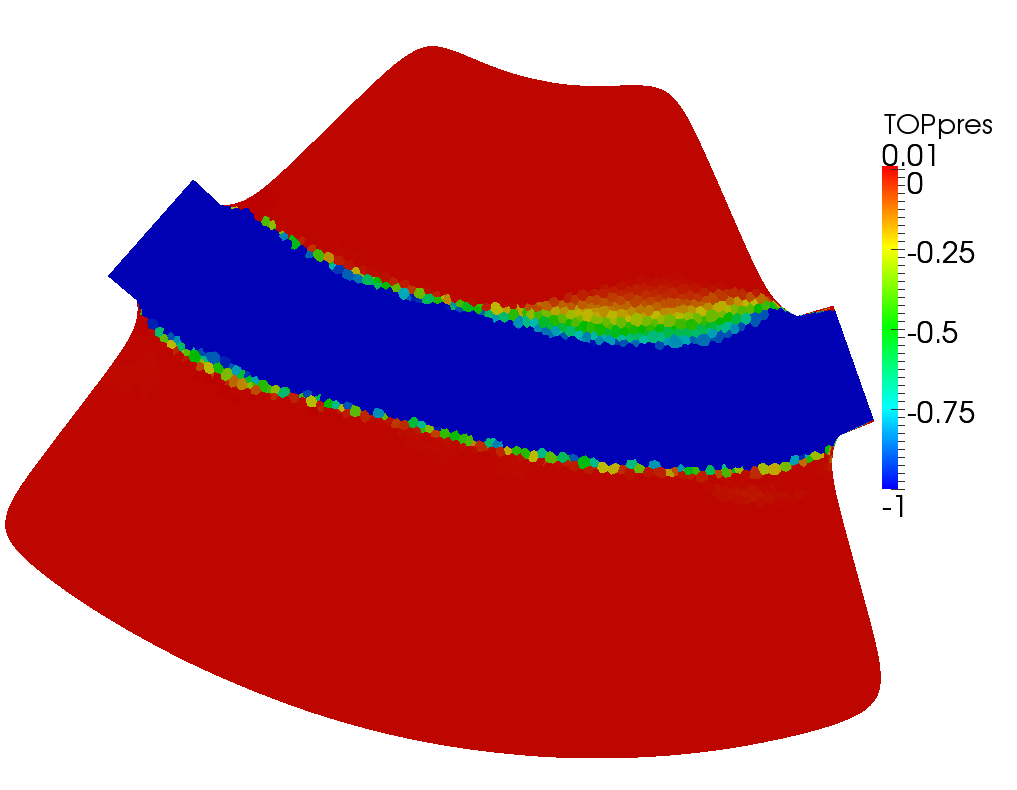
\includegraphics[scale=0.1]{TS2e5top.png}
    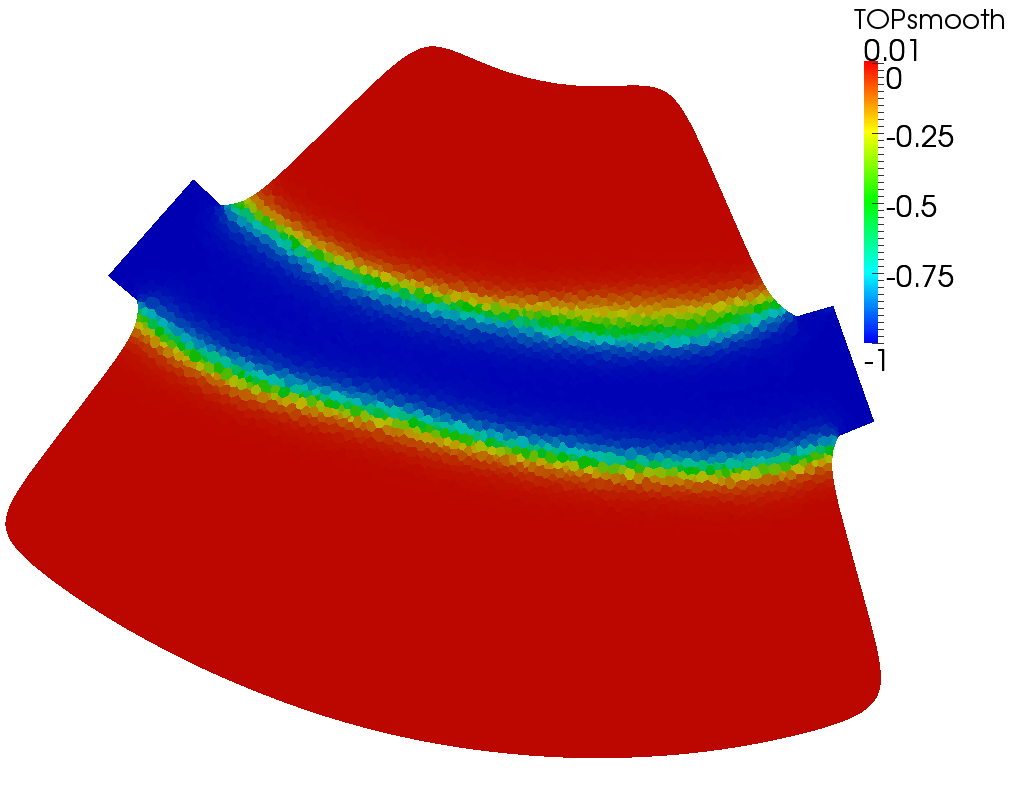
\includegraphics[scale=0.1]{TS2e5smooth.png}
    \caption{Left: $\TT\left(\bxx\right)$, \quad middle: $\overline{\TT}\left(\bxx\right)$, \quad right: $\TT_\sigma\left(\bxx\right)$.} 
    %\newline \textcolor{white}{.} \qquad \qquad \qquad
    %Unten: Topologieopt. Geom. (2.38e-5) und formopt. Geom. (aktuell:1.59e-5).}
    \label{Topo20}
\end{figure}
%
\begin{eqnarray}
\overline{\TT}\left(\bxx\right)=\mbox{min}\left(\mbox{max}\left(\TT\left(\bxx\right),\TT_{min}\right),\TT_{max}\right),
\end{eqnarray}
%
\begin{eqnarray}
- \sigma \Delta \TT_\sigma + \TT_\sigma &=& \overline{\TT} \qquad \mbox{in} \; \; \Om,\\
\TT_\sigma &=& \TT_{min} \quad \mbox{auf} \; \; \Gamma_i \cup \Gamma_o,\\
\partial_n \TT_\sigma &=& 0 \qquad \, \mbox{auf} \; \; \Gamma_w \cup \Gamma_f.
\end{eqnarray}
The parameters $\mathcal{T}_{\min}$ and $\mathcal{T}_{\max}$ are to be specified by the user with \texttt{cutTOP}. The smoothing parameter $\sigma$ must be set with \texttt{smoothTOP}. To avoid possible overlaps with the fixed geometries, the parameter \texttt{feasibleTOP} can be used to define the allowable range (see Figure \ref{extract3}).
\begin{figure}[htbp]
    \centering
    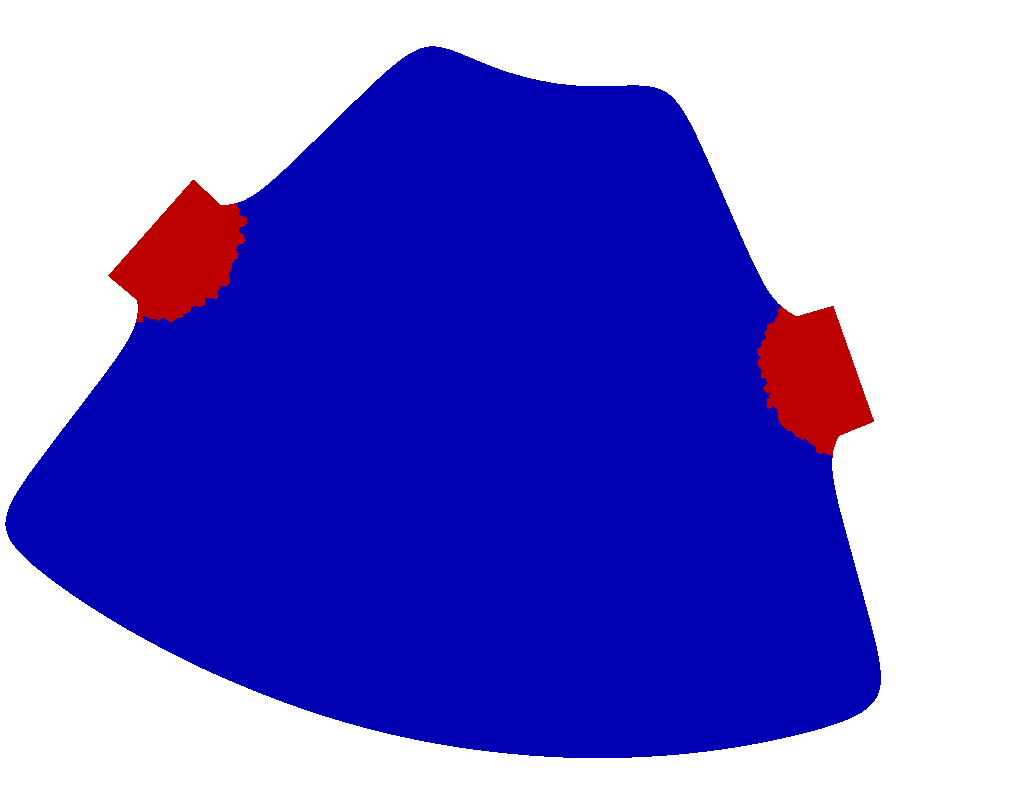
\includegraphics[scale=0.1]{TS2e5feasible.png}
    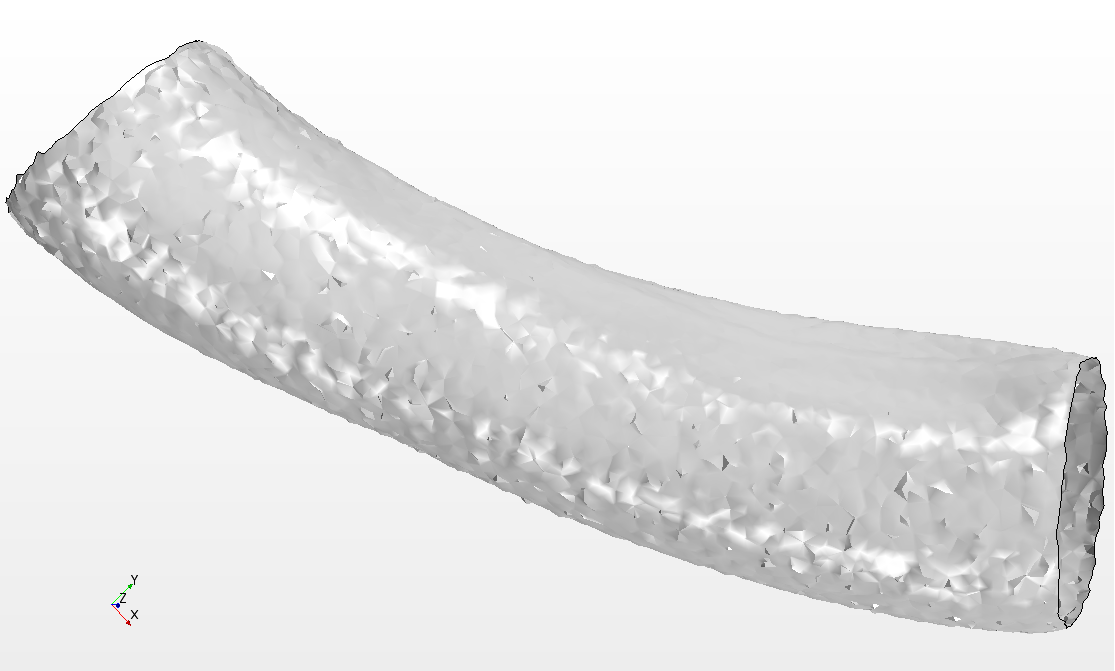
\includegraphics[scale=0.1]{TS2e5expSTL.png}
    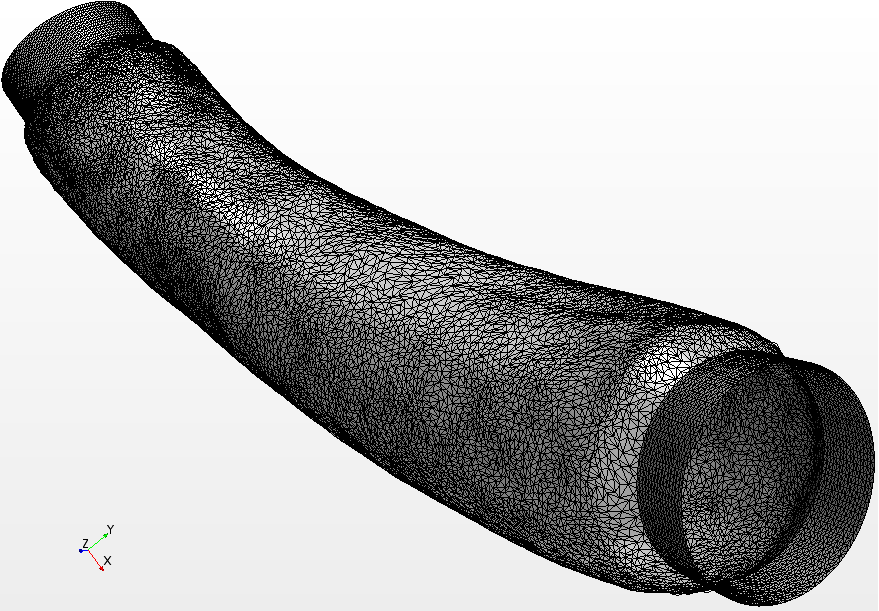
\includegraphics[scale=0.12]{TS2e5close2.png} 
    \caption{Left: Inadmissibility area (red); extracted geometry: middle: \emph{wallExtract.stl}, right: \emph{wall.stl}}
    \label{extract3}
\end{figure}
To allow the user to change the parameters quickly, the topoExtractSTL routine lists the default values and provides an input option. The parameters can also be changed in \texttt{system/fvSolution/SGparameter}.
\begin{table}[h]
    \centering
    \begin{tabular}{|p{2cm}|p{1cm}|p{1.6cm}|p{1.5cm}|p{4.4cm}|} %lcrp
        \hline
        \cellcolor{light-gray} Parameter name & \cellcolor{light-gray} Default value & \cellcolor{light-gray} Admissibility & \cellcolor{light-gray} B135 & \cellcolor{light-gray} Description\\
        \hline
        grad\_por          & 0      &  \{0,1\}                & 0          & 0: use TOPpres; 1: use PORalpha.\\
        \hline
        extractFolder      & 1      &  \{0,1e4\}              & 60         &  Extract geometry from folder with this number.\\
        \hline
        cutTOP             & 2(0 0) &  \{0,1\}                & 2(-1,0.01) & Maximum and minimum value.\\
        \hline
        smoothTOP          &   0    &  [0,1e5]                & 0.003      & Laplace smoothing the top degrees. information.\\
        \hline
        feasibleTOP        & 2(0 0) &  [0,1e6]                & 2(0 0)     & Range of inadmissibility at the in-/outlet in meters.\\
        \hline
        thresholdTOP       &   0    &  [-1e6,1e6]             & -0.5       & Level layer to achieve the surface.\\
        \hline
        %
    \end{tabular}
    \caption{Extraction of the topology optimized surface.}\label{tab:parameter10b}
\end{table}
$ $
\newpage
\section{Initialization and calculation}

\subsection{Executing the shape optimization}
\begin{itemize}
    \item Create a folder e.g. M23Test in \verb|$FOAM_RUN/tutorials/incompressible/|.
    \item In the folder M23Test the file \verb|parameter_sg| with the parameters and the folder \verb|initial_stl| with the geometry data must be created.
    \item From the folder M23Test the commands \texttt{setupShapeGradientCCM} and then
    \texttt{shapeGradientCCM > outtestShape.txt}.
\end{itemize}

\subsection{Executing the topology optimization}
\begin{itemize}
    \item Create a folder B135Test in \verb|$FOAM_RUN/tutorials/incompressible/|.
    In folder B135Test the file \verb|parameter_sg| with the parameters and the folder \verb|initial_stl| with the geometry data is to be created.
    \item The commands \texttt{setupShapeGradientCCM} and \texttt{topoOpt > outtestTop1.txt} must be executed from the B135Test folder. This returns TOPpres and PORalpha.
    \item From the M23Test folder the commands \texttt{topoExtractSTL} and \texttt{topoOptCloseAll > outtestTop2.txt} must be executed. This returns the intermediate result \texttt{wallExtract.stl} and the result \texttt{wall.stl}.
\end{itemize}

\subsection{Stop and restart shape optimization}
At the beginning of the shape optimization the file STOP.txt is automatically created. If the shape optimization is to be stopped, the number in the file must be changed to 0. During the shape optimization the subfolder sim is created in the iteration number folders where a mesh re-connection was performed. Together with the start geometries inlet.stl, outlet.stl, fixed.stl and if necessary bds.stl, wall.stl can be used for a new test calculation.

If the geometry change with respect to the start geometry is to be calculated, it must be saved in the \texttt{wall0.stl} file in the \verb|initial_stl| folder and the \verb|restart_opt| parameter must be set to 1 (see Table \ref{tab:parameter9}). If the same scaling of the target functionals is desired, the parameter \texttt{damp} must be specified in the \verb|parameter_sg| file. These values are always stored in the \verb|Test Run_Info.txt| file.

\section{Data evaluation and visualization}

\subsection{Output data}
During shape and topology optimization, the relevant data (see tables \ref{tab:output1} and \ref{tab:output2}) are stored in the corresponding folders (designation according to the number of iterations) in each iteration. The current geometry data is stored in \texttt{polyMesh}. Further data such as target function values, used step sizes, etc. can be found in the text file \verb|Testlauf_Info.txt|.

\begin{table}[h]
    \centering
    \begin{tabular}{|p{1.8cm}|p{1.4cm}|p{1.9cm}|p{6cm}|} %lcrp
        \hline
        \cellcolor{light-gray} Output file & \cellcolor{light-gray} Dimension & \centering \cellcolor{light-gray} Appearance &  \cellcolor{light-gray} Description \\
        \hline
        \centering U0          & \centering Vector     & \centering Area, boundary &      Solution $\buu$ the primary equation (velocity).\\
        \hline
        \centering p0          & \centering Scalar     & \centering Area, boundary &      Solution $ p$ of the primary equation (pressure).\\
        \hline
        \centering density0    & \centering Scalar     & \centering Area, boundary & Used density in the Navier-Stokes equation.\\
        \hline
        \centering Vunif       & \centering Vector     & \centering Area, boundary &      Solution $\bvv$ the adjoint equation (adjoint velocity) with regard to achieving a uniform flow.\\
        \hline
        \centering Vpres       & \centering Vector     & \centering Area, boundary &      Solution $\bvv$ the adjoint equation (adjoint velocity) with regard to minimizing the total pressure loss.\\
        \hline
        \centering Sg0u        & \centering Scalar     & \centering Boundary   &      Negative shape gradient (scaled).\\ 
        \hline
        \centering Sg00u       & \centering Scalar     & \centering Boundary   &      Negative shape gradient (scaled): proportion of $\JJ_1$, $\JJ_2$.\\ 
        \hline
        \centering Sg0Lu       & \centering Scalar     & \centering Boundary   &      Negative shape gradient (scaled): proportion geometric restriction.\\ 
        \hline
        \centering SgVpres0    & \centering Scalar     & \centering Boundary   &      Negative shape gradient (scaled): portion of $\JJ_2$ (total pressure loss).\\ 
        \hline
        \centering SgVunif0    & \centering Scalar     & \centering Boundary   &      Negative shape gradient (scaled): portion of $\JJ_1$ (uniform discharge).\\ 
        \hline
        \centering GeomChange  & \centering Scalar     & \centering Boundary   &      Geometry change to the initial geometry (in meters).\\     
        \hline
        \centering Distance    & \centering Scalar     & \centering Boundary   &      Distance to the installation space geometry (in meters).\\
        \hline
        \centering Sg0Pu       & \centering Scalar     & \centering Boundary, Point &      Negative shape gradient - Laplace-Beltrami (scaled).\\ 
        \hline
    \end{tabular}
    \caption{Output data shape optimization.}\label{tab:output1}
\end{table}
%
\begin{table}[h]
    \centering
    \begin{tabular}{|p{1.8cm}|p{1.4cm}|p{1.5cm}|p{6.2cm}|} %lcrp
        \hline
        \cellcolor{light-gray} Output file & \cellcolor{light-gray} Dimension & \centering \cellcolor{light-gray} Appearance &  \cellcolor{light-gray}  Description  \\
        \hline
        \centering TOPpres     & \centering Scalar     & \centering Area &      Topological sensitivity Total pressure loss.\\
        \hline
        \centering TOPmix      & \centering Scalar     & \centering Area &      Effective topological sensitivity.\\
        \hline
        \centering PORalpha    & \centering Scalar     & \centering Area &      Porosity.\\
        \hline
        \centering 1/TOPsmooth & \centering Scalar     & \centering Area &      Smoothed data $\TT_\sigma$ (\textbf{smoothTOP}).\\
        \hline
        \centering 1/TOPfea    & \centering Scalar     & \centering Area &      Admissibility range (\textbf{feasibleTOP}).\\
        \hline
    \end{tabular}
    \caption{Output data topology optimization.}\label{tab:output2}
\end{table}

\subsection{Visualization with ParaView}
For visualization of the data the use of ParaView is recommended. After installation in the course of the OpenFOAM setup paraView can be called with the command \emph{paraFOAM} in the folder with the data to be visualized. The following possibilities of data visualization can be used in paraView (see figure \ref{fig:paraview} - \ref{fig:paraviewTopo}) 
\begin{itemize}
    \item \emph{Point Field} and \emph{Volume Field} information on the surface (Sg0P, GeomChange), vector field with \emph{Glyph} (U0),
    \item cross-section with \emph{clip} or \emph{Slice} or contour with \emph{Contour} (TOPpres, PORalpha, TOPsmooth),
    \item STL data with \emph{File$>$Open} (wallExtract.stl).
\end{itemize}

\begin{figure}[h]
    \centering
    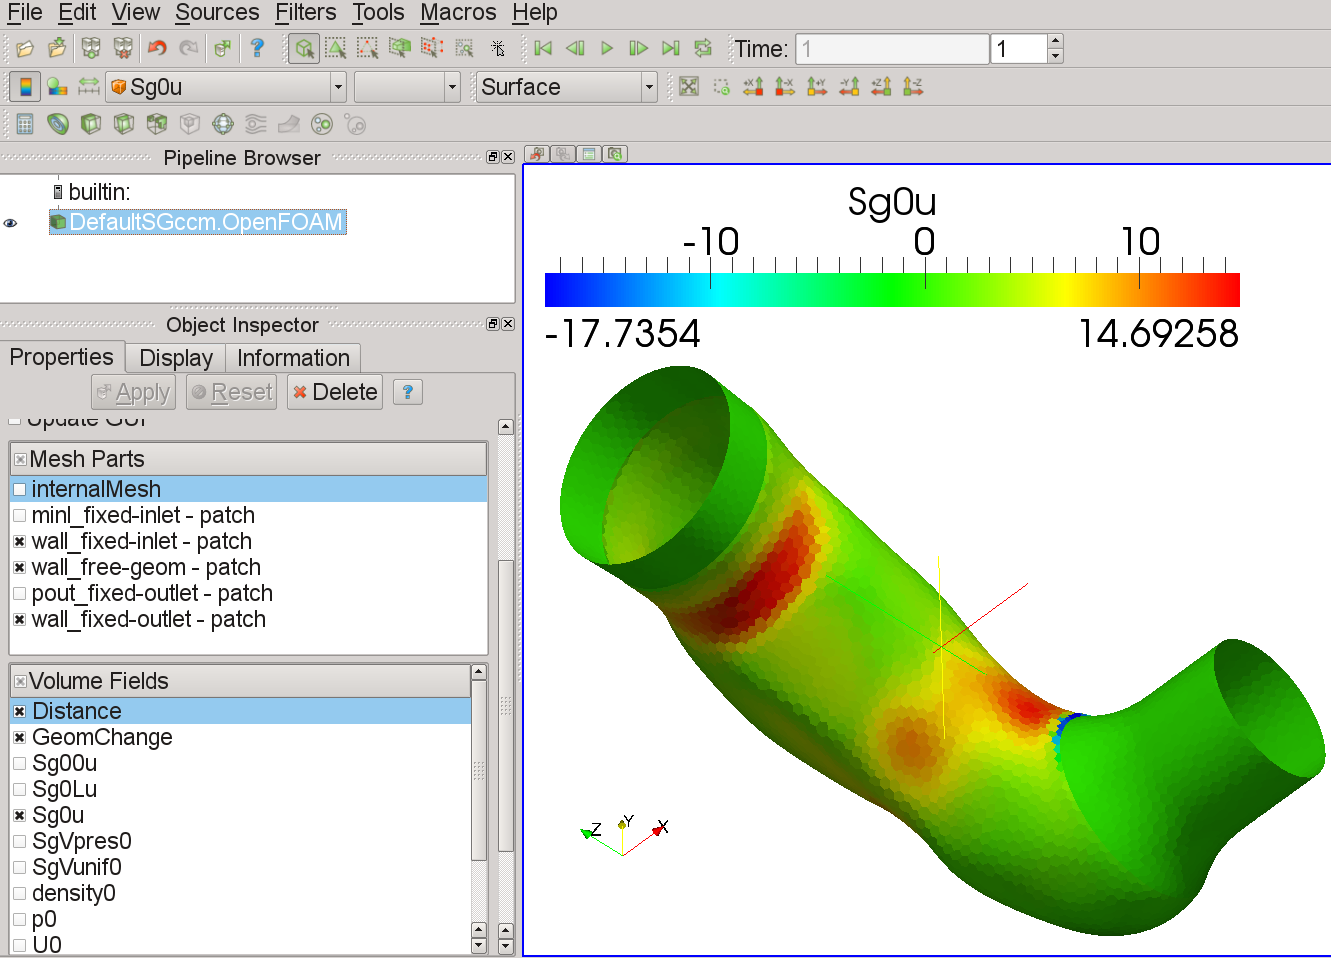
\includegraphics[scale=0.23]{paraview1.png}
    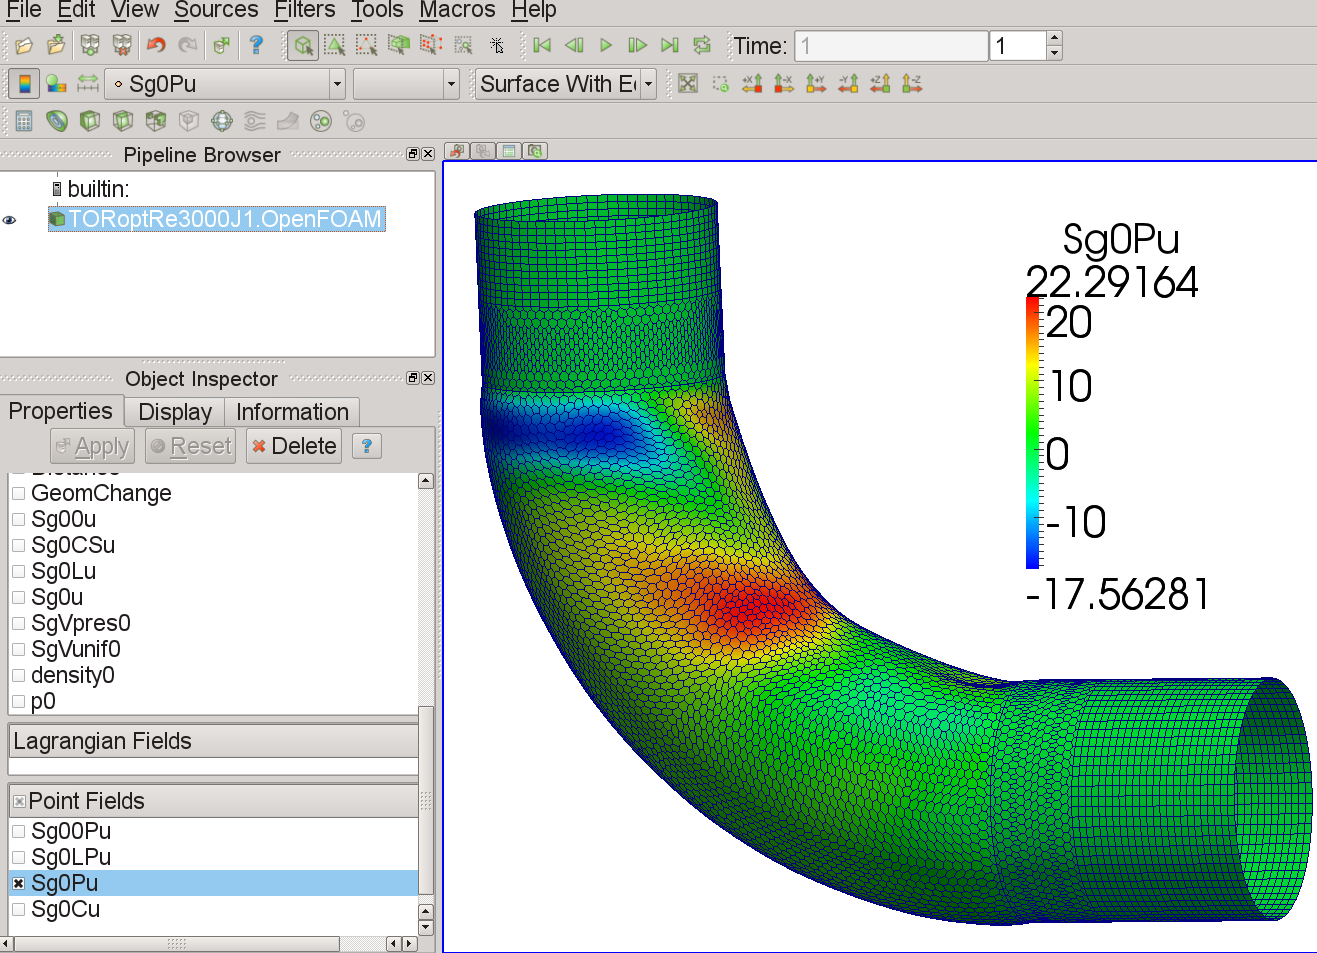
\includegraphics[scale=0.23]{paraview3.png}
    \caption{Use of ParaView: VolumeFields, PointFields.} 
    \label{fig:paraview}
\end{figure}

\begin{figure}[htbp]
    \centering
    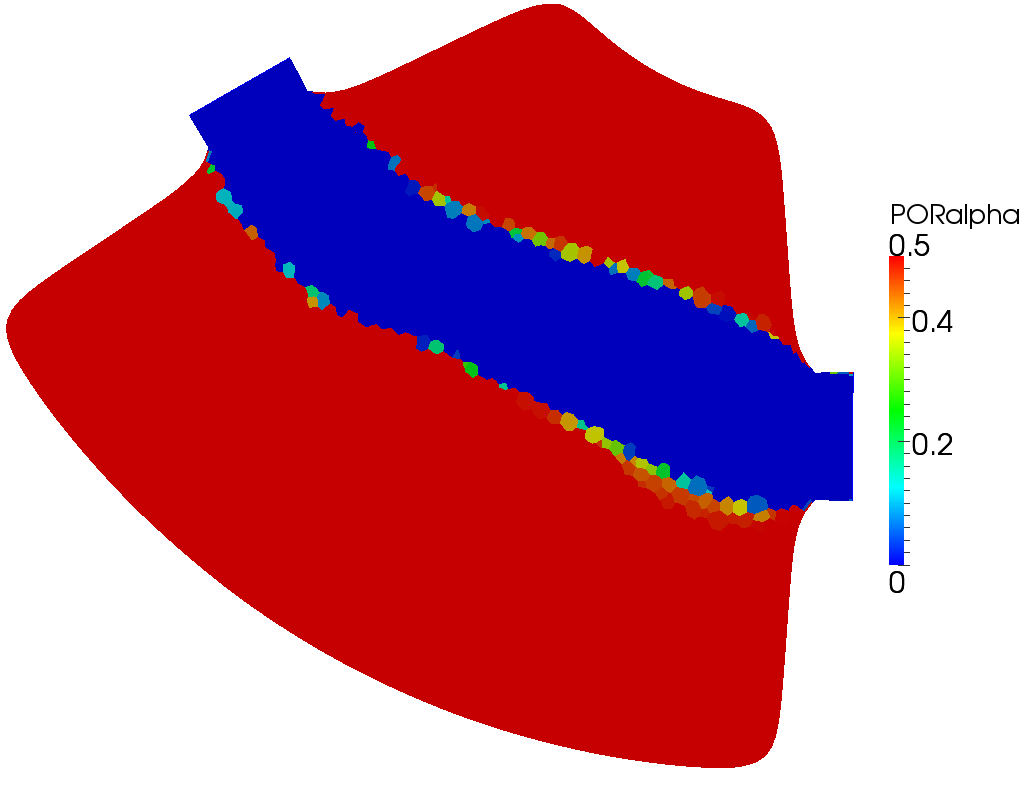
\includegraphics[scale=0.11]{S200por8.png}
    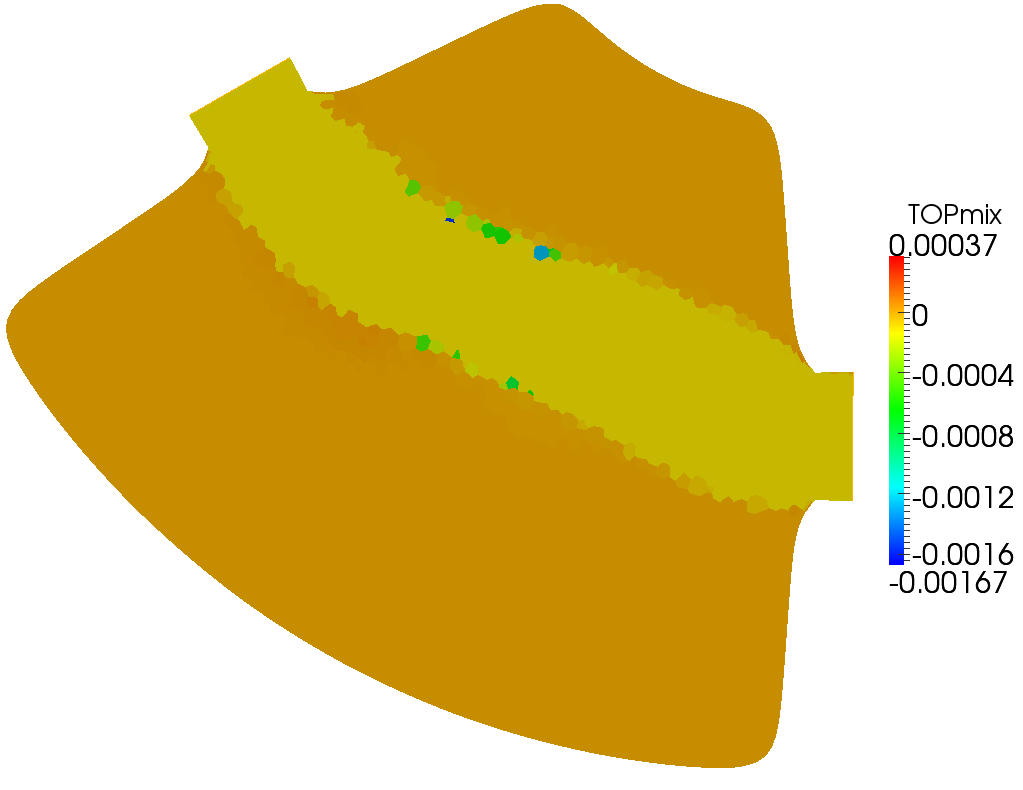
\includegraphics[scale=0.11]{S200top7.png}
    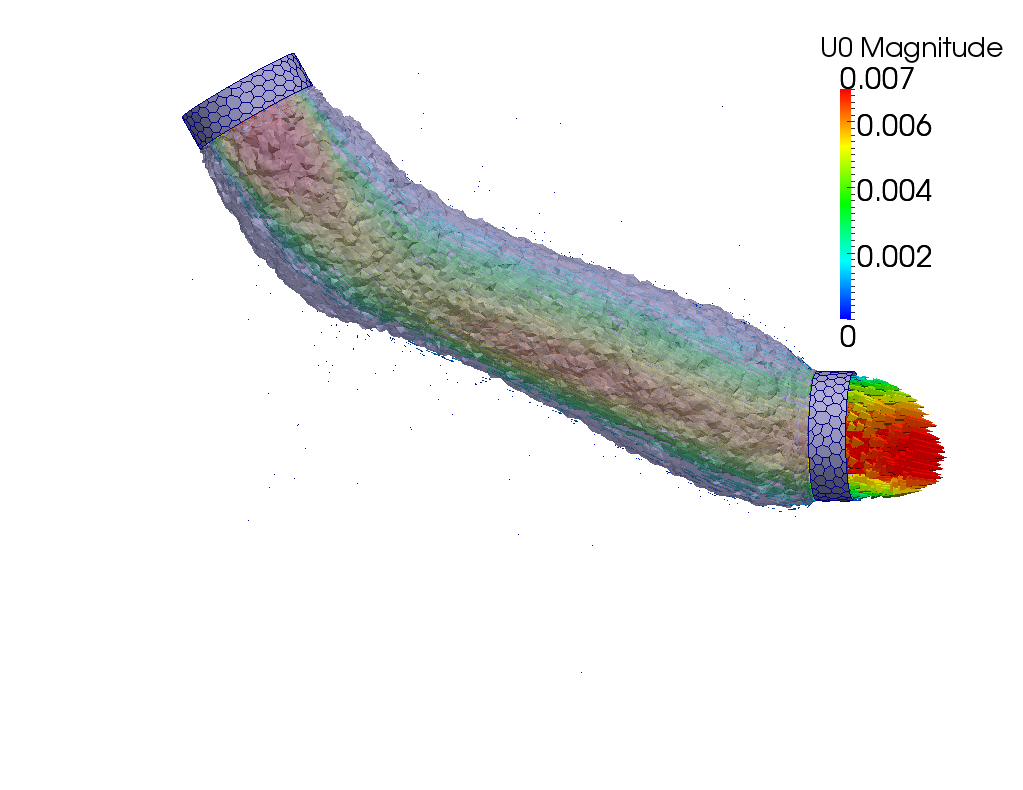
\includegraphics[scale=0.11]{S200con7.png}
    \caption{Porosity, effective top. degree and contour.} 
    \label{fig:paraviewTopo}
\end{figure}
%
\begin{landscape}
    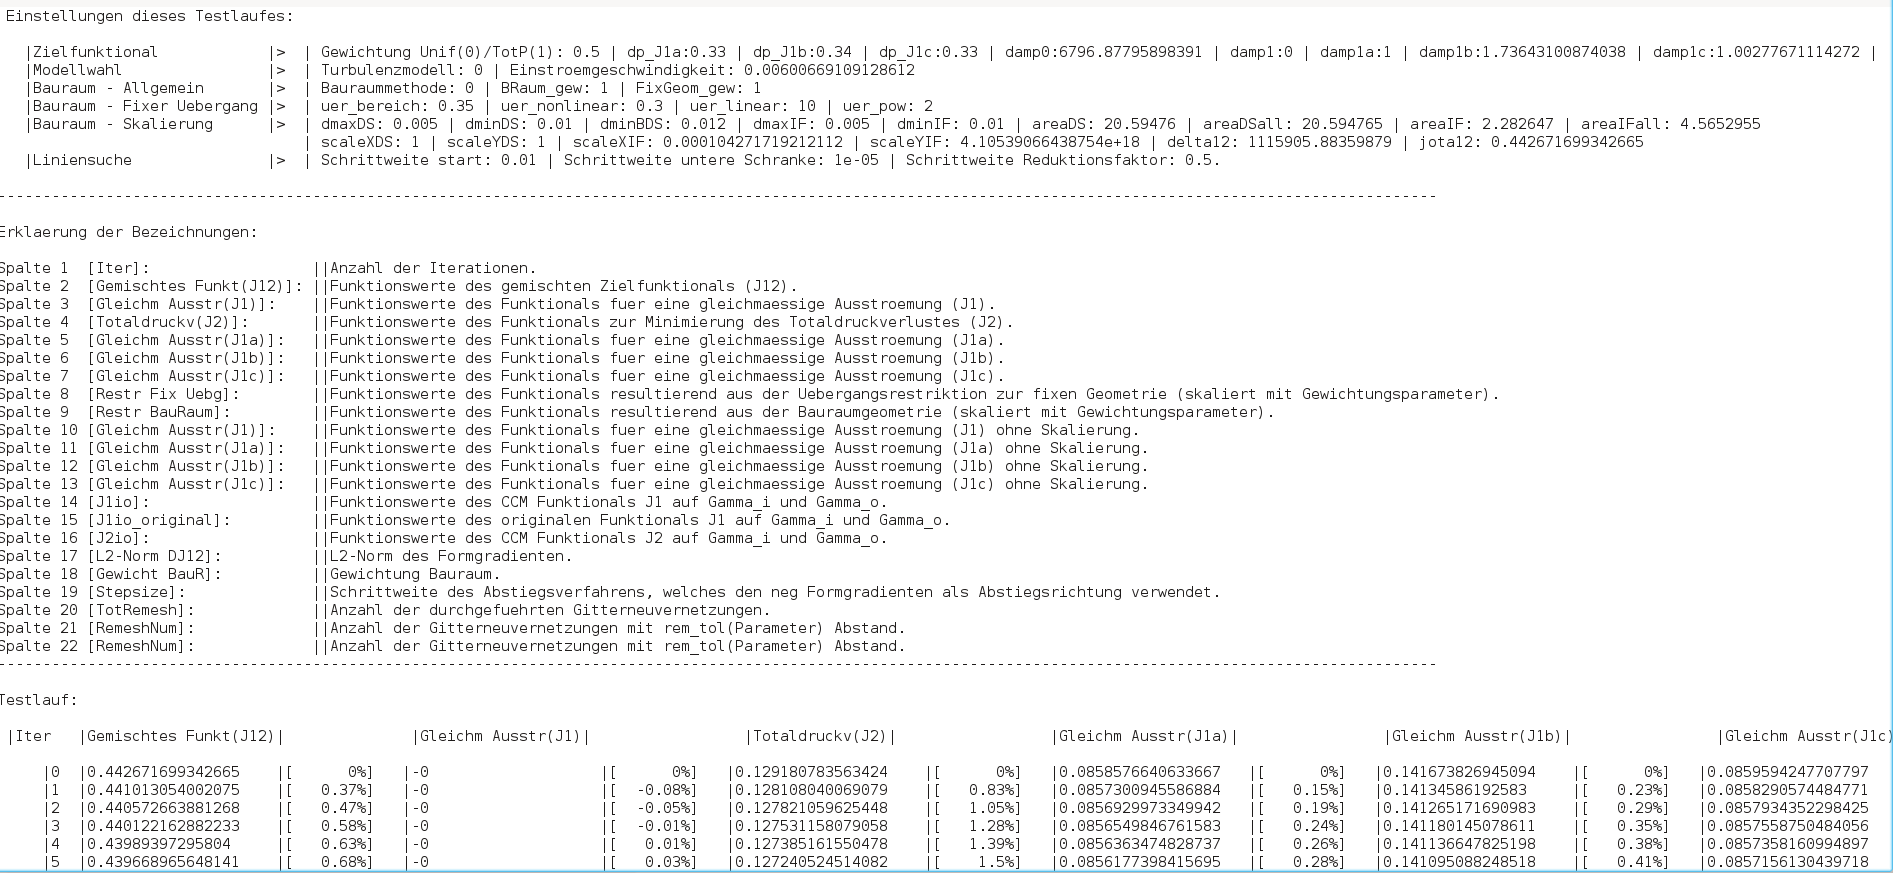
\includegraphics[scale=0.5]{testlauf_info161.png}\\
    $ $\\ 
    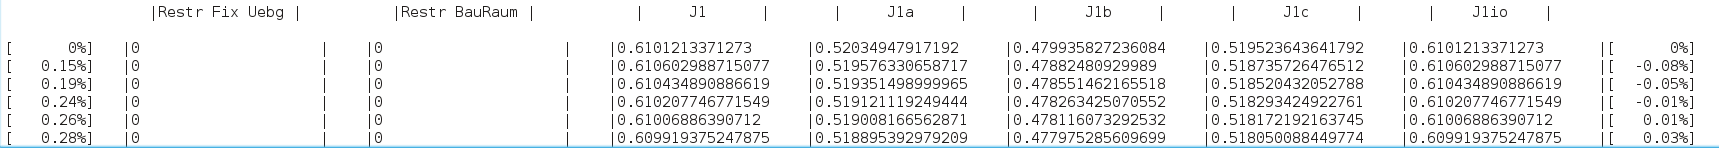
\includegraphics[scale=0.5]{testlauf_info162.png}\\
    $ $\\ 
    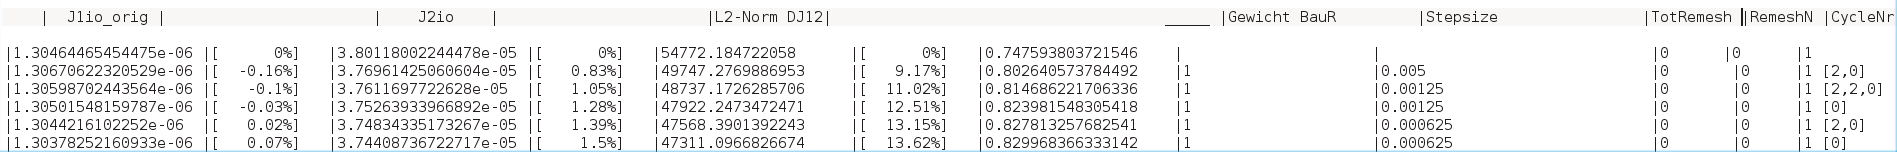
\includegraphics[scale=0.5]{testlauf_info163.png}
\end{landscape}

\subsection{Structure diagram}
A software structure chart is shown in figure \ref{fig:struktogramm}.
Calculation steps are shown in square fields and queries in rounded fields.
The essential software parts are shown in grey letters for the respective calculation steps.
In the output file \emph{test run\_Info.txt}, a numerical code is located in square brackets at the end of the line of each iteration.
This numerical code indicates the progress of the step size control within the respective iteration.\\
The digits can be found in the structure diagram in figure \ref{fig:struktogramm}, their meaning is given in table \ref{tab:zahlencode}.

\begin{table}[h]
    \centering
    \begin{tabular}{|p{0.8cm}|l|} %lcrp
        \hline
        \cellcolor{light-gray} Digit & \cellcolor{light-gray} Meaning \\
        \hline
        0             & Step accepted/end of iteration.\\
        \hline
        1             & Grid Networking.\\
        \hline
        2             & Grid quality criteria not fulfilled for entire geometry .\\
        \hline 
        3             & Installation space exceeded when using the barrier method.\\
        \hline
        33            & Installation space overrun of the start geometry when using barrier method.\\
        \hline
        4             & Target functional does not fall according to Armijo - rule.\\
        \hline
        6             & Primary solver does not converge.\\
        \hline
        66            & Primary solver does not converge at startup configuration.\\
        \hline
        7             & Grid quality criteria not met for geometry \emph{wall}.\\
        \hline
        8             & Surface quality insufficient.\\
        \hline
        9             & User enforced reconnection.\\
        \hline
    \end{tabular}
    \caption{Number code line search shape optimization.}\label{tab:zahlencode}
\end{table}

\begin{figure}[htbp]
    \centering
    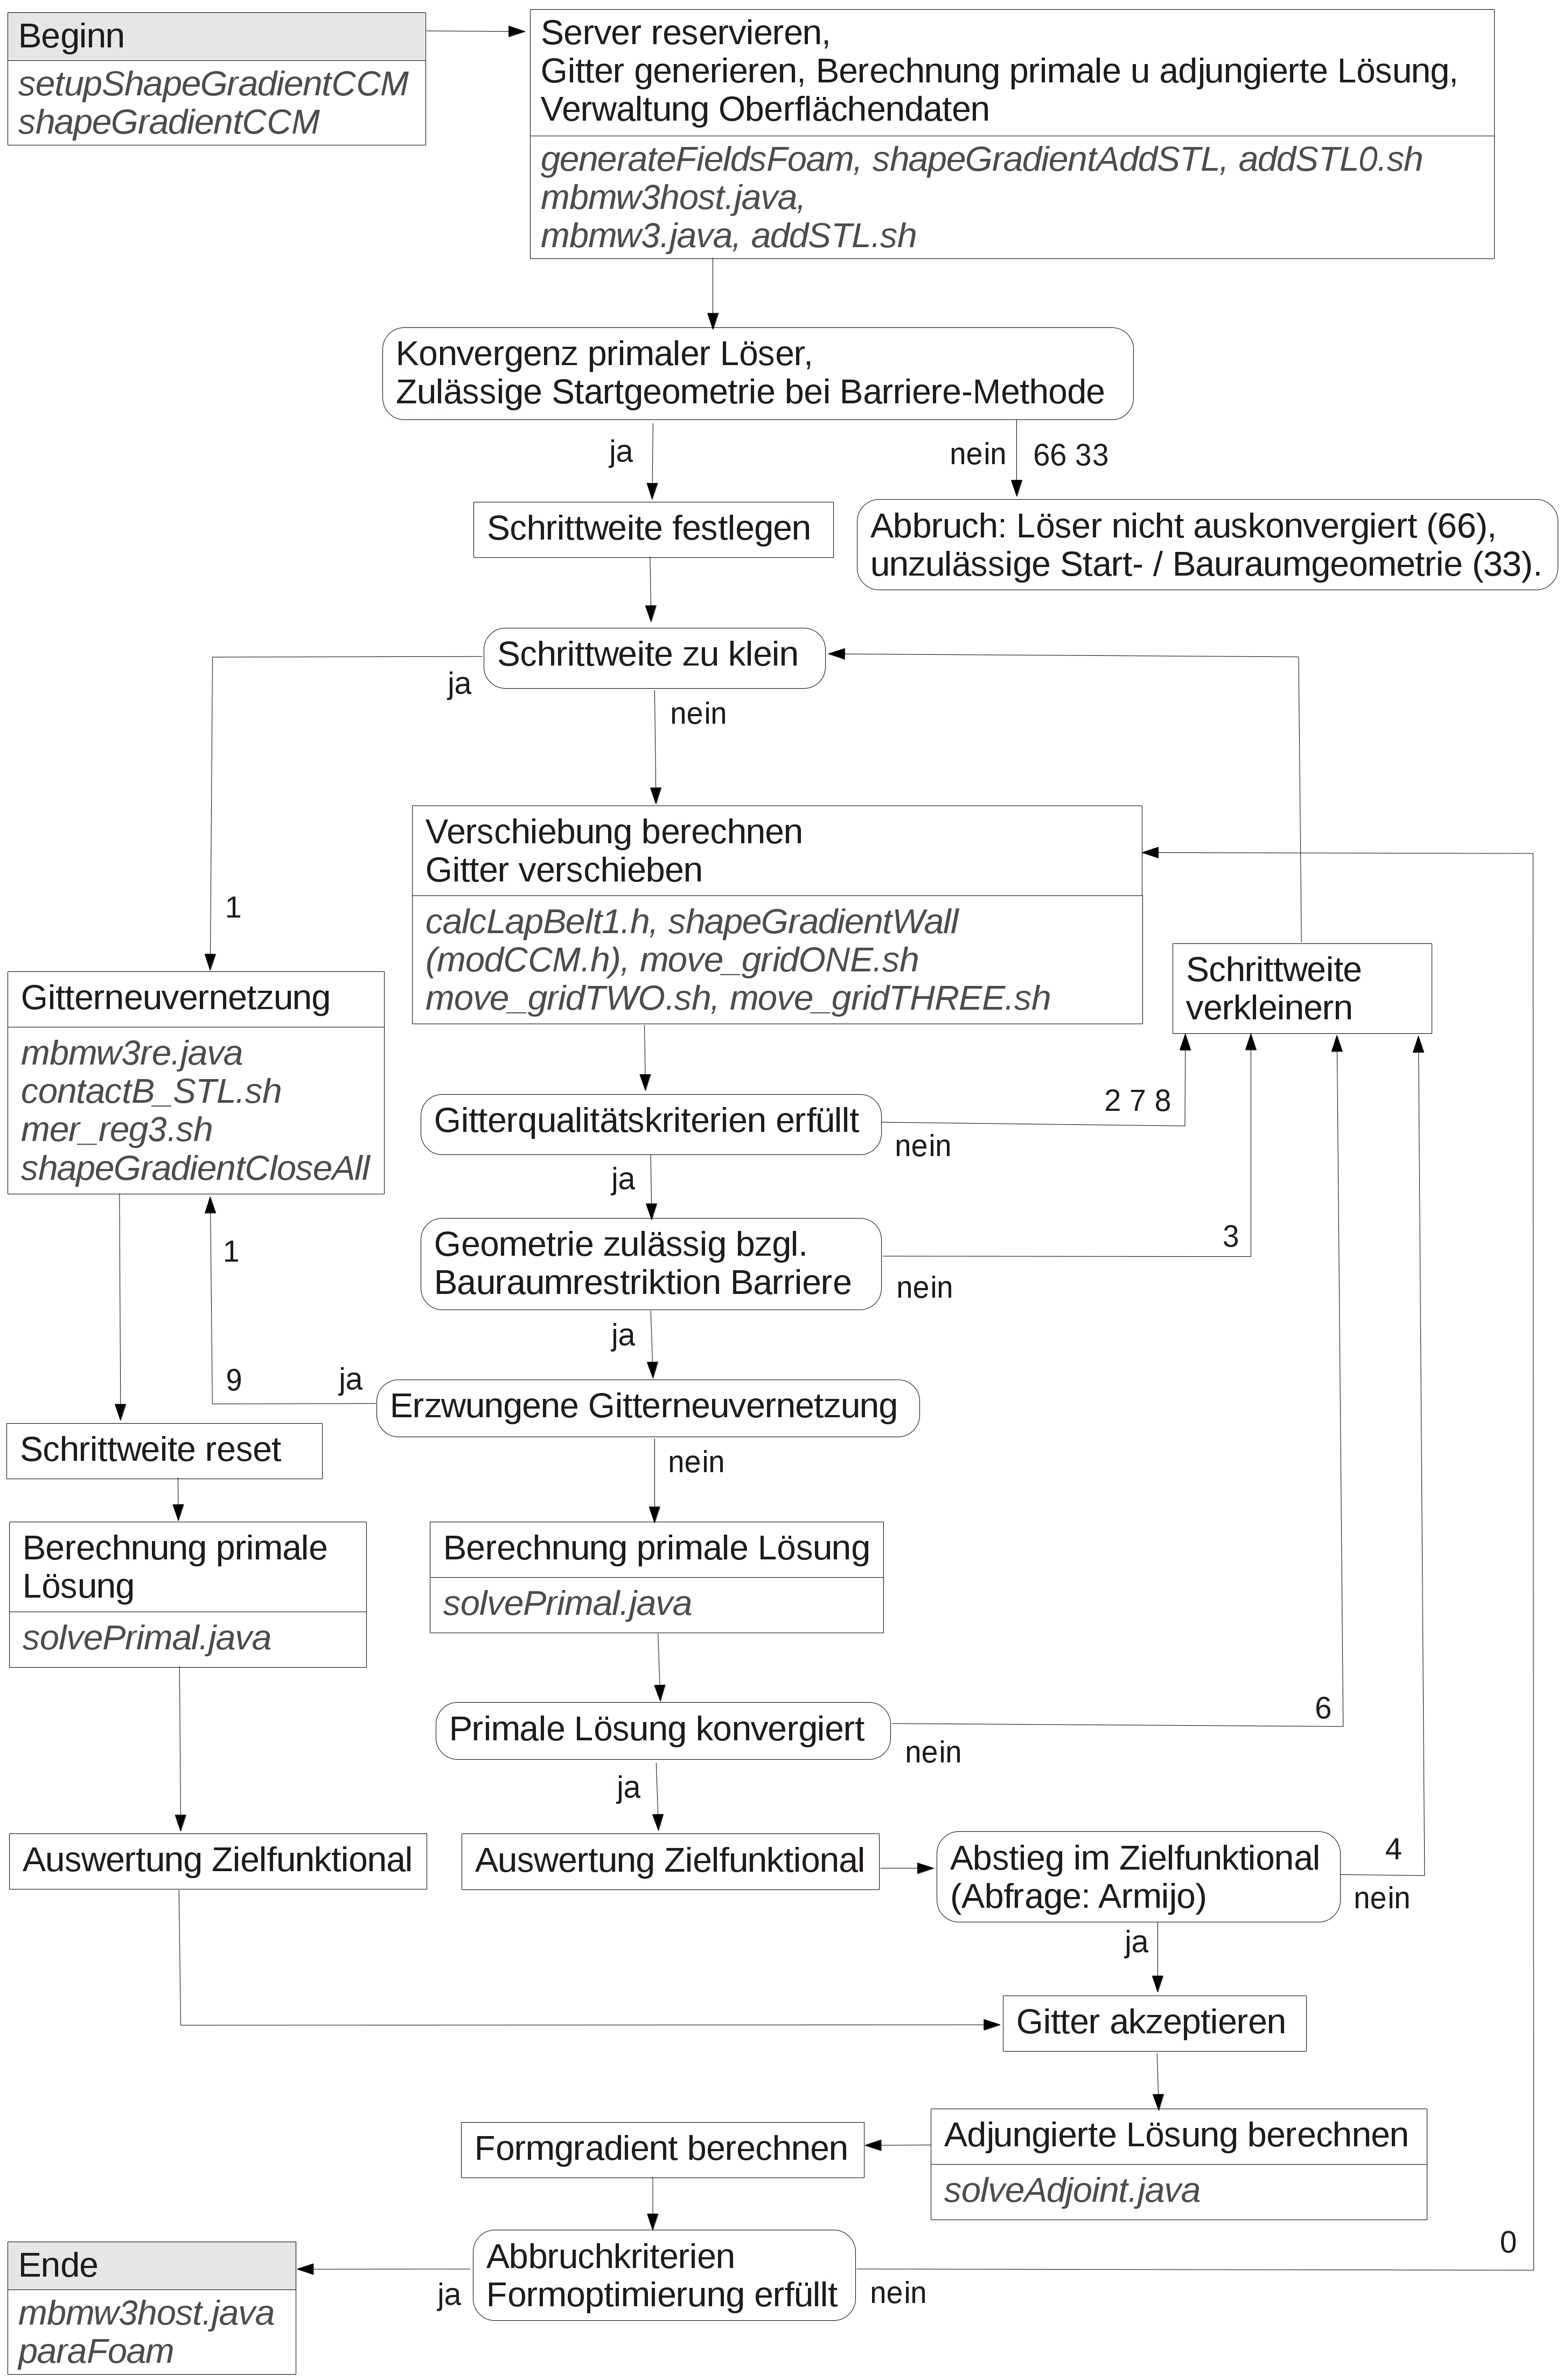
\includegraphics[scale=0.47]{struktogramm16.png}
    \caption{Structogram shape optimization.} 
    \label{fig:struktogramm}
\end{figure}


\printbibliography[heading=bibintoc]
\end{document}